\documentclass[10pt,openany]{book}
\usepackage{verbatim}
\usepackage{enumerate}
\usepackage{float}
\usepackage{tabularx}
\usepackage{multirow}
\usepackage{lmodern}
\usepackage{rotating}

%\usepackage[pdftex]{color}
%\usepackage[final]{pdfpages}

\usepackage{graphicx}
\graphicspath{ {./images/} }


\usepackage{minitoc}\usepackage{minitoc} 
\renewcommand{\mtifont}{\large\sffamily}
\renewcommand{\mtcfont}{\small\sffamily}
\renewcommand{\mtcSfont}{\small\sffamily}
\renewcommand{\mtcSSfont}{\small\sffamily}
\renewcommand{\mtcSSSfont}{\small\sffamily}

%\renewcommand{\familydefault}{lmodern}

\usepackage[a5paper,bindingoffset=0.2in,%
            left=0.75in, right=0.5in, top=0.75in,bottom=1.0in,
            footskip=.5in, headheight = 1in]{geometry}

\usepackage{fancyhdr}

\pagestyle{fancy}
\fancyhf{}
\fancyhead[LE,RO]{\leftmark }   %was \leftmark {Section number\\Section Title}
\fancyhead[RE,LO]{\bfseries Van's Aircraft\\RV7} %manufacturer masthead nextline and airplane model series
\fancyfoot[LE,RO]{\thepage} %section number - page number
\fancyfoot[RE,LO]{\today}  %original issuer or date of revision


\usepackage[auto]{chappg}
\usepackage[ddmmyyyy]{datetime} 
\usepackage[english]{babel}
\addto\captionsenglish{\renewcommand{\chaptername}{Section}}  

%this calls chapters sections as gama likes it
\setcounter{secnumdepth}{0}  %this avoids numbering underneath sections eg. 3.1.1

\renewcommand{\familydefault}{\sfdefault}

%\title{'RV-7 POH'}
%\author{P.P.A. Kotze}

\usepackage{tikz}
\newcommand*\circled[1]{\tikz[baseline=(char.base)]{
            \node[shape=circle,draw,inner sep=2pt] (char) {#1};}}



\begin{document}
%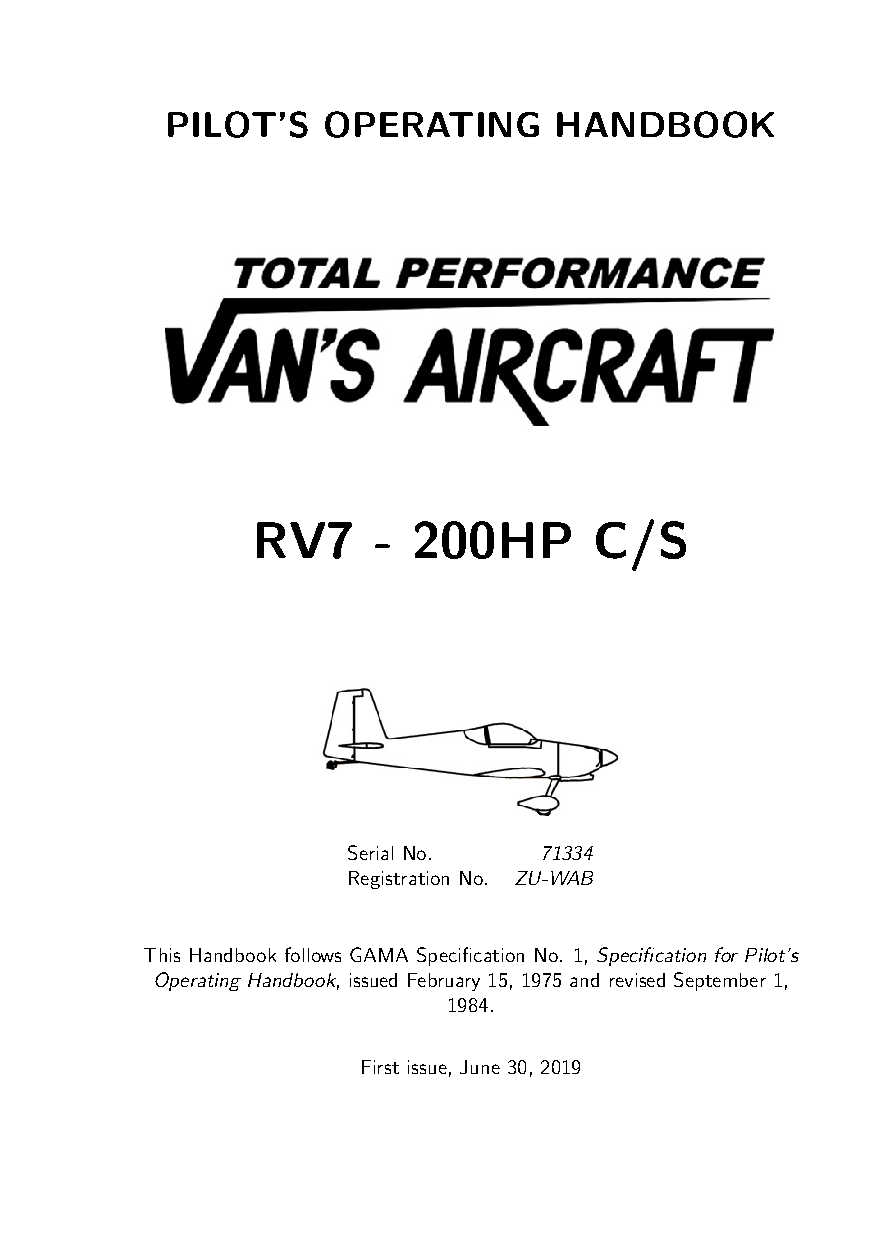
\includepdf[pages=-,nup=1x2,landscape,signature=explain]{/home/pkotze/RV7POH/zuwab.pdf}

\dominitoc% Initialization
\pagenumbering{Roman}
%\chapter{General}
\thispagestyle{empty}

\begin{center}


\textbf{\LARGE{PILOT'S OPERATING HANDBOOK 
\\[0.5in]
}
}
\end{center}

\begin{figure}[h]
\centering

\includegraphics[width=1\textwidth]{vans-aircraft-logo.eps}
\label{fig:logo}
\end{figure}

\begin{center}

\textbf{\Huge{RV7 - 200HP C/S}}\\[0.5in]
\end{center}

\begin{figure}[H]
\centering
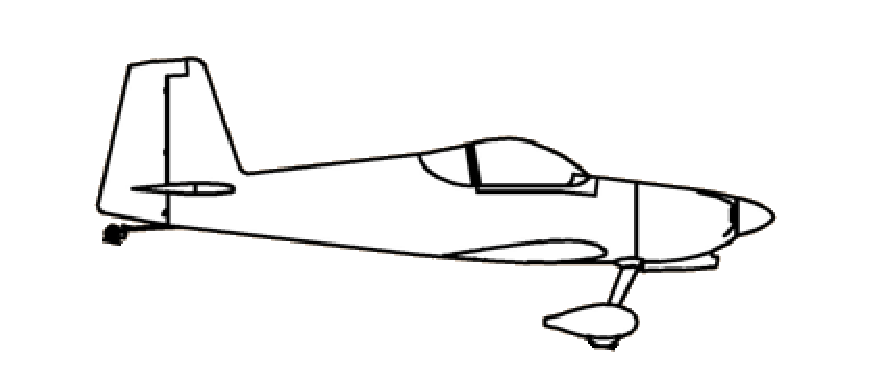
\includegraphics[height=0.15\textheight]{cover_rv.eps}
\end{figure}

\begin{center}
\begin{tabular}{ l r }
Serial No. & \textit{71334} \\ 
Registration No. & \textit{ZU-WAB} \\[0.25in]
\end{tabular}
\end{center}


\begin{center}
%THIS HANDBOOK INCLUDES THE MATERIAL REQUIRED TO BE FURNISHED TO THE PILOT BY THE REGULATIONS AND ADDITIONAL INFORMATION PROVIDED BY THE MANUFACTURER AND CONSTITUTES THE APPROVED AIRPLANE FLIGHT MANUAL.  \\[0.25in]

This Handbook follows GAMA Specification No. 1, \textit{Specification for Pilot's Operating Handbook}, issued February 15, 1975 and revised September 1, 1984.\\[0.25in]

First issue, \today
\end{center}









%\chapter{Performance Specifications}
%Wronge name I know....
\thispagestyle{fancy}

\textbf{RV7 Performance}\\

\begin{tabularx}{\linewidth}{
    >{\hsize=0.7\hsize}X
    >{\hsize=0.15\hsize}X
    >{\hsize=0.15\hsize}X  }
WEIGHT\\
Solo Weight \dotfill &1400 lbs&\\
Gross Weight \dotfill &1800 lbs&\\
\\
SPEED - Solo Weight\\
Top Speed\dotfill               & 188 kt\\
Cruise [75\% @ 8000 ft]\dotfill	& 180 kt\\
Cruise [55\% @ 8000 ft]\dotfill & 162 kt\\
Stall Speed\dotfill	            & 45 kt\\
SPEED - Gross Weight\\
Top Speed\dotfill	            & 187 kt\\
Cruise [75\% @ 8000 ft]\dotfill	& 179 kt\\
Cruise [55\% @ 8000 ft]\dotfill	& 161 kt\\
Stall Speed\dotfill	            &  51 kt\\
\\ 	
GROUND PERFORMANCE\\
Ground Performance - Solo Weight	\\
Takeoff Distance\dotfill	&250 ft\\
Landing Distance	\dotfill&350 ft\\
 	
Ground Performance - Gross Weight\\
Takeoff Distance	\dotfill&500 ft\\
Landing Distance	\dotfill&500 ft\\
\\
CLIMB/CEILING\\ 	
Climb/Ceiling - Solo Weight	
Rate of Climb\dotfill	&2,550 fpm\\
Ceiling\dotfill	&25,500 ft\\
 	
Climb/Ceiling - Gross Weight	
Rate of Climb\dotfill	&1,900 fpm\\
Ceiling\dotfill	&22,500 ft\\
\\ 	
RANGE\\
Range [75\% @ 8000 ft]\dotfill	664 nm\\
Range [55\% @ 8000 ft]\dotfill	812 nm\\
\end{tabularx}

\begin{center}
NOTE\\
Numbers in this table are provided by the kit manufacturer and are not measured performance on the aircraft identified on the front page.  
The speeds and ranges indicatged are converted from claimed numbers in mph or statute miles to knots or nautical miles.
\end{center}  %one page performance specifications
%\chapter{REVISIONS}
\thispagestyle{fancy}

\begin{center}
\textbf{PILOT's OPERATING HANDBOOK\\
LOG OF REVISIONS\\[0.25in]
}

  \begin{tabularx}{\linewidth}{
    |>{\hsize=0.25\hsize}X| 
    >{\hsize=0.25\hsize}X|
    >{\hsize=0.5\hsize}X| 
  }
 \hline
  Revision Number and Date & Revised Pages &  Description of Revision \\ 
 \hline
  1: 13/07/2018 & All & Initial creation of document\\ 
 \hline
  2: 28/11/2018 & Systems & Tyre and tube detail added\\ 
 \hline
  3: 20/12/2018 & Equipment list & Equipment list added\\ 
 \hline
  4: 29/01/2019 & Weight \& balance & Actual numbers used  \\ 
 \hline
                & Systems & Moved Equipment list to Systems\\ 
 \hline
                & Systems & Added EFIS backup battery\\ 
 \hline
  5: 20/10/2019 & Performance  & Add engine performance \\ 
 \hline
                & Normal Operations & Update speeds\\ 
 \hline
  &  & \\ 
 \hline
  &  & \\ 
 \hline
  &  & \\ 
 \hline
  &  & \\ 
 \hline
\end{tabularx}

\end{center}  %Added from GAMA spec
%\maketitle
\tableofcontents
%\thispagestyle{empty} 

\pagenumbering{arabic}
\pagenumbering{bychapter}
\chapter{General description}
\thispagestyle{fancy}
\minitoc[n] % Creating an actual minitoc

\section{General}
This pilot's operating handbook is designed  to provide information relevant to achieve maximum utilisation 
of the aircraft.  It is not designed to be a substitute for adequate and competent flying instruction 
and should not be used for operational purposes unless kept up to date.

Assurance that the aircraft is airworthy is the responsibility of the owner.  The pilot in command is responsible for
ensuring the aircraft is safe for flight and for operating within the limits detailed in this handbook and as displayed on placards and instrument markings in the aircraft.

\section{Three View}
The RV7 is a propeller driven conventional gear aircraft with a wingspan of 7.7m, a length of 6.1m and a height of 1.6m as shown in Figure~\ref{fig:rv-7_3view}.

\begin{figure}[H]
\centering
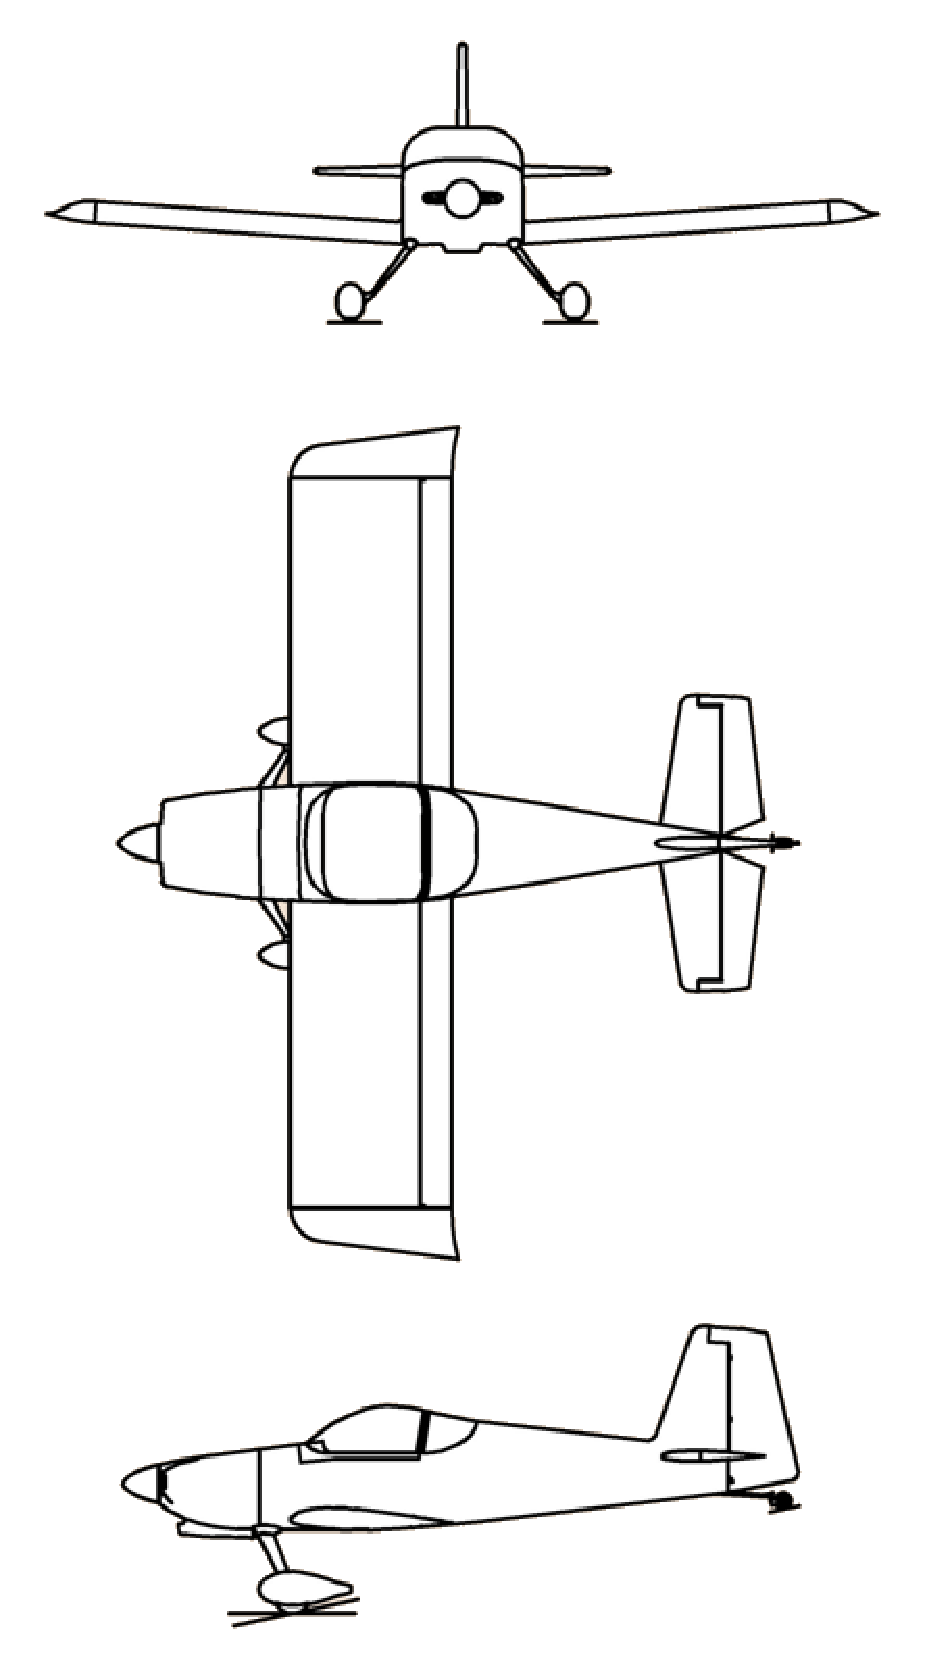
\includegraphics[height=0.5\textheight]{rv-7_3view.eps}
\caption{RV7 three view: Wingspan 7.7m, Length 6.1m, Height 1.6m}
\label{fig:rv-7_3view}
\end{figure}

\section{Descriptive Data}
\subsection{Engine}
%Four cylinder air-cooled, horizontally opposed, direct drive, fuel injected, tuned induction engine having oil jets for internal piston cooling.  Provisions for single action controllable pitch propeller.  Impulse coupling magnetos.  Crankshaft equipped with one 6.3 order and one 8th order counterweights.

\begin{tabularx}{\linewidth}{
  >{\hsize=0.4\hsize}X
  >{\hsize=0.6\hsize}X  }
 Number of Engines: & 1  \\ 
 Engine manufacturer: & Avco Lycoming  \\  
 Engine Type: & Normally-aspirated, air-cooled, horizontally opposed, fuel injected, four-cylinder engine\\
 Engine Model number: & IO-360-A1B6\\
 Rated horespower: & 200 hp\\
 Rated speed, RPM: & 2700 rpm \\
 Displacement, cu inch: & 361.0\\
 Compression ratio: & 8.7:1 \\
 Firing order: & 1-3-2-4 \\
 Propeller rotation: & Clockwise \\
 Weight: & 333 lbs \\

\end{tabularx}

\subsection{Propeller}
  \begin{tabularx}{\linewidth}{
    >{\hsize=0.4\hsize}X
    >{\hsize=0.6\hsize}X  }
Propeller Manufacturer: & Hartzell\\
Propeller Model No: & HC-C2YR-1BFP/F7497-2\\%HC - Hartzell controllable, C2YR C-Standard Hub, 2 - no. of blades, YR - Y shank aluminium blade, R - mounting flange, 
%1 CONSTANT SPEED, NO COUNTERWEIGHT OIL PRESSURE TO HIGH PITCH, BLADE CENTRIFUGAL FORCE TO LOW
%BFP B-830-21 STOP UNITS F-LARGE PITCH CHANGE KNOB, FORK
%F - large pitch change knob Y shank 
%74 - blade diameter next number spec model. 
Number of Blades: & 2\\
Propeller Diameter: & Maximum 72"\\ %% I believe we can say 72" here as it is exactly that.
Propeller Type: & Variable Pitch\\
Weight: & 51.8 lbs \\
Limitation: & None\newline (Type Certificate Data sheet No. P-920)\\
\end{tabularx}

\subsection{Fuel}
  \begin{tabularx}{\linewidth}{
    >{\hsize=0.4\hsize}X
    >{\hsize=0.6\hsize}X  }
Approved Fuel Grades: & 100/130 Aviation Fuel (Blue).\\
Capacity: & 42 US Gal (159$\ell$)\\
Useable fuel: & 40 US Gal (151$\ell$)\\ % Could be as high as 41.94 but should be measured
Max fuel pressure: & 12psi (CHECK THIS)\newline  (>9psi indicates possible blocked injector)\\
\end{tabularx}

\subsection{Oil}
  \begin{tabularx}{\linewidth}{
    >{\hsize=0.4\hsize}X
    >{\hsize=0.6\hsize}X  }
Oil capacity: & 8 US Qt (min 2 US Qt) \\
\end{tabularx}

\subsection{Maximum Weights}
  \begin{tabularx}{\linewidth}{
    >{\hsize=0.4\hsize}X
    >{\hsize=0.6\hsize}X  }
Maximum weight: & 1800 lbs (820 kg)\\
Max baggage weight: & 100 lbs (45 kg) \\

\end{tabularx}

\subsection{Standard airplane weights}
  \begin{tabularx}{\linewidth}{
    >{\hsize=0.4\hsize}X
    >{\hsize=0.6\hsize}X  }
Standard empty weight: & 1122 lbs (510 kg)\\
Usable load: & 679 lbs (310kg) \\
\end{tabularx}

\subsection{Cabin and Entry dimensions}
The cabin features side by side seating with control and  brakes for both occupants.   Cabin entry is made through the open canopy by stepping from the wing over the cabin side onto the seat.

\subsection{Baggage space and entry dimensions}
Baggage is stored behind the seatbacks of the front occupants.  A maximum weight of 100 lbs and volume of 12 cubic feet is available for baggage.

\subsection{Specific loadings}
  \begin{tabularx}{\linewidth}{
    >{\hsize=0.4\hsize}X
    >{\hsize=0.6\hsize}X  }
Wing Loading: & 14.8 lb/sq ft\\
Power Loading: & 9.0 lb/hp \\
\end{tabularx}

\section{Symbols}
  \begin{tabularx}{\linewidth}{
    >{\hsize=0.2\hsize}X
    >{\hsize=0.8\hsize}X  }
$V_a$    & Manoeuvring speed. Speed at which full application of aerodynamic control will not overstress the aircraft. \\
$V_{fe}$ & Maximum Flap Extension Speed. Highest Speed permissible with wing flaps in a prescribed extended position. \\
$V_{ne}$ & Never exceed speed. Not to be exceeded at any time. \\
$V_{no}$ & Maximum structural cruising speed. Not to be exceeded except in smooth air and then only with caution.\\ 
$V_{s}$  & Stalling speed. The minimum steady airspeed at which the aircraft is controllable. \\
$V_{so}$ & Stalling speed. The minimum steady airspeed at which the aircraft is controllable, in the landing configuration. \\
$V_x$    & Best angle of climb. Airspeed that delivers greatest altitude gain in shortest horizontal movement. \\
$V_y$    & Best rate of climb. Airspeed delivering greatest altitude gain in shortest possible time.\\
\end{tabularx}

\section{Abbreviations}
  \begin{tabularx}{\linewidth}{
    >{\hsize=0.2\hsize}X
    >{\hsize=0.8\hsize}X  }
CAS & Calibrated airspeed. Indicated airspeed corrected for position and instrument error. Equates to true airspeed in standard atmosphere at sea level. \\
%KCA & CAS in” Knots” \\
GS & Groundspeed. Speed relative to the ground \\
IAS & Indicated Airspeed. Speed, as shown on Airspeed indicator, includes instrument and position error. \\
KIAS & IAS in Knots \\
kt & Knots \\
NM & Nautical Miles\\
TAS & True airspeed relative to undisturbed air, which is the CAS, corrected for altitude, temperature and pressure. \\
\end{tabularx}

\section{Terminology}
  \begin{tabularx}{\linewidth}{
    >{\hsize=0.2\hsize}X
    >{\hsize=0.8\hsize}X  }
%Accelerate-Stop Distance: & Distance to accelerate to a specified speed and, assuming engine failure when that speed is attained, bring the aircraft to a stop. \\
Constant Speed & A propeller system which employs a governing device to maintain a selected engine RPM.\\
Demonstrated crosswind & Demonstrated cross wind component for which adequate control of the aircraft during take off and landing has been demonstrated.\\
Empty Weight & Weight of the airplane including fixed ballast, unusable fuel and oil.\\
Gross Weight & Sum of empty weight plus crew, passengers, fuel and baggage.  \\
Maximum Gross Weight & The maximum allowable operating weight with all variable load items located such that the Centre of Gravity remains within prescribed limits.\\
Payload & Weight of passengers and baggage.\\
Useful Load & Weight of passengers, fuel and baggage.\\
\end{tabularx}


\chapter{Limitations}
\thispagestyle{fancy}
\minitoc[n] % Creating an actual minitoc

\section{Introduction}
This section includes operating limitations, instrument markings and basic placards necessary for the safe operation of the aircraft, its engine, standard systems and equipment.

\section{Airspeed Limitations}
\begin{table}[h]
\caption{Airspeed Limitations}
\label{tab:airspeed_limits}
%\begin{tabular}{ |p{0.5in}|p{2.5in}|p{0.5in}|p{2in}| } 
  \begin{tabularx}{\linewidth}{
    |>{\hsize=0.08\hsize}X| 
     >{\hsize=0.4\hsize}X|
     >{\hsize=0.12\hsize}X| 
     >{\hsize=0.5\hsize}X| 
  }
   \hline
  &SPEEDS &KIAS &REMARKS\\ 
 \hline
 $V_{NE}$ & Never exceed speed & 200 kt & Do not exceed this speed in any operation\\ 
 \hline
 $V_{NO}$ & Maximum structural cruising speed & 168 kt & Do not exceed this speed except in smooth air, and then only with caution\\ 
  \hline
 $V_{A}$ & Manoeuvering Speed & 123 kt & Do not make full or abrupt control movements above this speeds \\ 
  \hline
%  {$V_{FE}$}  & \shortstack[l]{Maximum Flap Extended Speed: \\To 20$^{\circ}$ Flaps\\ 20$^{\circ}$ - 40$^{\circ}$ Flaps} & \shortstack[l]{\\96 \\ 87} & Do not exceed these speeds with the given flap settings \\ 
% \hline
  {$V_{FE}$}  & Flap Extended Speed: \newline To 20$^{\circ}$ Flaps \newline 20$^{\circ}$ - 40$^{\circ}$ Flaps & - \newline 96 kt \newline 87 kt & ~\newline Do not exceed these speeds  with the given flap settings \\ 
 \hline
\end{tabularx}
\end{table}

\section{Airspeed Indicator Markings}
\begin{table}[H]
\caption{Airspeed Indicator Markings}
\label{tab:airspeed_indicator}
  \begin{tabularx}{\linewidth}{
    |>{\hsize=0.15\hsize}X| 
     >{\hsize=0.25\hsize}X|
     >{\hsize=0.6\hsize}X| 
} 
 \hline
  MARKING & KIAS VALUE or  RANGE &  SIGNIFICANCE \\ 
 \hline
 White Arc & 51 kt - 87 kt& Full flap operating range.  Lower limit is maximum weight $V_{S0}$ in landing configuration.  Upper limit is maximum speed permissible with flaps extended.\\ 
 \hline
 Green Arc & 56 kt - 168 kt & Normal operating range.  Lower limit is maximum weight $V_{S}$ with flaps retracted.  Upper limit is maximum structural cruising speed.\\ 
 \hline
 Yellow Arc & 168 kt - 200 kt& Operations must be conducted with caution and only in smooth air. \\ 
 \hline
 Red Line  & 200 kt & Maximum speed for all operations \\ 
 \hline
\end{tabularx}
\end{table}

\section{Power plant limitations}
Engine Operating Limits for Takeoff and Continuous Operations:

\begin{tabularx}{\linewidth}{
    >{\hsize=0.5\hsize}X
    >{\hsize=0.5\hsize}X
  }
 Engine manufacturer: & Avco Lycoming\\  
 Engine Model number: & IO-360-A1B6\\
 Maximum Power: & 200 hp\\
 Maximum Engine Speed: & 2700 RPM\\
 Maximum Cylinder Head Temp: & 500$^{\circ}$F \textit{(260$^{\circ}$C)} \\
 Maximum Oil Temperature: & 245$^{\circ}$F \textit{(118$^{\circ}$C)}\\
% Oil Pressure: & 25 to 95 psi\\
 Oil Pressure: & 125 psi\\
 Fuel Pump Pressure: & -2 - 35 psi \\
 Fuel Injector Pressure: & 14 - 45 psi \\
 Propeller Manufacturer: & Hartzell\\
 Propeller Model No: & HC-C2YR-1BFP/F7497-2\\
 Propeller Diameter: & Maximum 72"\\
 Propeller Blade Angles: & Low: 13.6$^{\circ}$\newline High: 35$^{\circ}$\\
\end{tabularx}

\section{Power plant instrument markings}
Power plant instrument marking and their colour code significance are shown in Table \ref{tab:eng_limits}.  The limits tabled are based on the Lycoming engine operating manual. To maximise engine service life green arc limits should be adhered to and engine power settings of 65\% or less is recommended.

\begin{table}[H]
\caption{Power Plant Instrument Markings}
\label{tab:eng_limits}
\begin{tabularx}{\linewidth}{
    |>{\hsize=0.24\hsize}X| 
     >{\hsize=0.18\hsize}X|
     >{\hsize=0.19\hsize}X| 
     >{\hsize=0.20\hsize}X| 
     >{\hsize=0.19\hsize}X|  
     } 
\hline
\multirow{2}*{Instrument}      & Minimum Limit &Normal Operating & Caution Range &  Maximum Limit \\
\hline
& RED LINE &GREEN ARC & YELLOW ARC & RED LINE \\
% \hline
%& Minimum Limit & Normal Operating & Caution Range & Maximum Limit \\ 
% \hline
%  Instrument & RED LINE & GREEN ARC & YELLOW ARC & RED LINE\\ 
 \hline
%  Tachometer & \dotfill & 2100 - 2500 RPM & \dotfill & 2700RPM \\ 
  Tachometer & \dotfill & 1800 - 2500 RPM & \dotfill & 2700RPM \\ 
  \hline
  Manifold \newline Pressure & \dotfill & 15 - 25 \newline in. Hg & \dotfill & 28.7 \newline in. Hg \\ 
 \hline
  Oil \newline Temperature & 140$^{\circ}$F & 165 - 220$^{\circ}$F & \dotfill & 245$^{\circ}$F \\ 
 %  Oil \newline Temperature & 140$^{\circ}$F \newline \emph{60$^{\circ}$}C & 165$^{\circ}$-220$^{\circ}$F\newline  \emph{74$^{\circ}$-104$^{\circ}$C}  & \dotfill & 245$^{\circ}$F \newline \emph{118$^{\circ}$C}  \\ 
 \hline
  %Cylinder Head Temperature & 150$^{\circ}$F(66$^{\circ}$C)  & 150$^{\circ}$F(66$^{\circ}$C) to 400$^{\circ}$F(205$^{\circ}$C)  & 400$^{\circ}$F(205$^{\circ}$C) to 435$^{\circ}$F(224$^{\circ}$C) &  500$^{\circ}$F(260$^{\circ}$C)  \\ 
Cylinder Head \newline Temperature & 150$^{\circ}$F& 150 - 400$^{\circ}$F  & 400 - 435$^{\circ}$F &  500$^{\circ}$F \\ 
%Cylinder Head \newline Temperature & 150$^{\circ}$F\newline \emph{66$^{\circ}$C} & 150$^{\circ}$-400$^{\circ}$F \newline \textit{66$^{\circ}$-205$^{\circ}$C} & 400$^{\circ}$-435$^{\circ}$F \newline \textit{205$^{\circ}$-224$^{\circ}$C}&  500$^{\circ}$F\newline 260$^{\circ}$C \\ 
 \hline
% \hline
  Fuel Pressure (Flow) & -2 psi & -2 - 35 psi & \dotfill & 35psi \\ 
  \hline
  Oil Pressure  & 25 psi & 55 - 95 psi & \dotfill & 95/115psi\\ 
 \hline
\end{tabularx}
\end{table}

\section{Weight Limits}
  \begin{tabularx}{\linewidth}{
    >{\hsize=0.5\hsize}X
     >{\hsize=0.5\hsize}X
  }
 Maximum Takeoff Weight: & 1800 lbs  \\ 
 Maximum Landing Weight: & 1800 lbs  \\  
 Maximum Aerobatic Weight: & 1600 lbs  \\  
 Maximum Weight Baggage: & 100 lbs  \\  
\end{tabularx}

\section{Centre of Gravity limits}
Reference Datum: 70" forward of the leading edge of the wing. 
\subsection{Normal Operations}
Center of Gravity range:
\begin{itemize}
\item{Forward:} 78.7" aft of datum at 1800 lbs or less
\item{Aft:} 86.8" aft of datum at 1800 lbs or less
\end{itemize}

\subsection{Aerobatic Operations}
Center of Gravity range:
\begin{itemize}
\item{Forward:} 78.7" aft of datum at 1600 lbs or less
\item{Aft:} 84.5" aft of datum at 1600 lbs or less
\end{itemize}

\section{Manoeuvre limits}
This aircraft is designed for flight in both the normal and aerobatic category.
\subsection{Normal Category}
The normal category is applicable to aircraft intended for non-aerobatic operations.  These include manoeuvres incidental to normal flying, stalls (except whip stalls), lazy eights, chandelles and steep turns in which the angle of bank is not more than 60$^{\circ}$.

\subsection{Aerobatic Category}
The aerobatic category is applicable to the aircraft when loaded within limits.  Aerobatic manoeuvres include, Loops, Horizontal Eights, Immelman Turns, Aileron Rolls, Barrel Rolls, Snap Rolls, Vertical Rolls and Split S.

\section{Flight load limit factor limits}
\subsection{Normal Category}
At any weight between 1600lbs and 1800lbs or at any CG location aft of 84.5 inches, the aircraft flight load limits are +4.4 and -2.2G.

\subsection{Aerobatic Category}
At an Aerobatic gross weight of 1600lbs the airframe structure is designed to withstand indefinitely flight load limits of +6 and -3G.  

\section{Kinds of operation limits}
This aircraft is approved for any operation approved in accordance with the current Authority to Fly.

\section{Fuel limitations}
  \begin{tabularx}{\linewidth}{
    >{\hsize=0.4\hsize}X
    >{\hsize=0.6\hsize}X  }
Approved Fuel Grades: & 100/130 Aviation Fuel (Blue).\\
Capacity: & 42 US Gal (159$\ell$)\\
Useable fuel: & 40 US Gal (151$\ell$)\\
\end{tabularx}

\section{Placards}
The follwoing information is displayed in the form of composite or individual placards.

\begin{enumerate}[(1)]
\item At fuel valve (at appropriate locations):

  \begin{tabularx}{\linewidth}{
    >{\hsize=0.4\hsize}X
    >{\hsize=0.6\hsize}X  }
Fuel Total & 40 US Gal (151$\ell$)\\
Left Tank & 20 US Gal \\
Right Tank & 20 US Gal \\
\end{tabularx}

\begin{comment}
\item In full view of the pilot:
\begin{table}[h]
\caption{Aerobatic Entry Speeds}
\label{tab:aerobatic_speeds}
  \begin{tabularx}{\linewidth}{|
    >{\hsize=0.5\hsize}X|
    >{\hsize=0.25\hsize}X|
    >{\hsize=0.25\hsize}X|
  }
\hline
Manoeuvre: & Speed [mph] & Speed [kt]\\
\hline
Loops, Horizontal eights:&140 - 190 mph & 122 - 165 kt\\
\hline
Immelman Turns: & 150 - 190 mph & 130 - 165 kt\\
\hline
Aileron Rolls, Barrel Rolls: &120 - 190 mph & 104 - 165 kt\\
\hline
Snap rolls &80 - 110 mph & 70 - 96 kt\\ 
\hline
Vertical Rolls: &180 - 190 mph  & 156 - 165 kt\\
\hline
Split-S:       &100 - 110 mph & 87 - 96 kt\\
\hline
\end{tabularx}
\end{table}
\end{comment}

\end{enumerate}
\chapter{Emergency procedures}
\thispagestyle{fancy}
\minitoc[n] % Creating an actual minitoc

\section{Introduction}
This section provides checklist and amplified procedures for coping with emergencies that may occur.  Emergencies caused by airplane or engine malfunctions are extremely rare if proper preflight inspection and maintenance are practised.  

\section{Airspeeds for Emergency Operations}
\begin{table}[H]
\caption{Airspeed for Emergency Operations}
%\label{tab:airspeed_emergencies}
  \begin{tabularx}{\linewidth}{
    |>{\hsize=0.2\hsize}X| 
     >{\hsize=0.6\hsize}X|
     >{\hsize=0.2\hsize}X| 
} 
 \hline
   & Description &  Airspeed\\ 
   \hline
 $V_{ref}$ & Engine Failure After Take Off & 70 kt\\ %manoeuvre
  \hline
 $V_{glide}$ & Best glide & 78 kt  \\ 
   \hline
 $V_{a}$ & Manoeuvring speed & 123 kt \\ %manoeuvre
 \hline
\end{tabularx}
\end{table}


\section{ENGINE FAILURE}
\subsection{Engine Failure during Takeoff Run}
\begin{enumerate}[(1)]
  \item Throttle -- CLOSED
  \item Brakes -- APPLY
  \item Wing Flaps -- RETRACT
  \item Mixture -- IDLE CUT OFF
  \item Ignition -- OFF
  \item Master -- OFF
\end{enumerate}

\subsection{Engine Failure After Take Off}
\begin{enumerate}[(1)]
  \item Airspeed -- 78 KIAS
  \item Mixture -- IDLE CUT OFF
  \item Fuel Selector -- OFF
  \item Ignition -- OFF
  \item Flaps -- AS REQUIRED
  \item Master -- OFF
\end{enumerate}

\subsection{Engine Failure During Flight}
\begin{enumerate}[(1)]
  \item Airspeed -- 78 KIAS
  \item Fuel Selector -- SWITCH TANKS
  \item Mixture -- RICH 
  \item Fuel pump -- ON 
  \item Ignition -- ON
\end{enumerate}

  If power not restored

\begin{enumerate}[(a)]
\item Ignition  -- Cycle OFF then ON
\item Alternate Air -- PULL
\item Throttle and Mixture -- RESET
\end{enumerate}

 If power not restored perform Forced Landing.

\section{FORCED LANDING}
\subsection{Emergency Landing without Engine power}
\begin{enumerate}[(1)]
  \item Airspeed -- 78 KIAS
  \item Fuel Selector -- OFF
  \item Mixture -- IDLE CUT OFF
  \item Ignition -- OFF
  \item Flaps -- AS REQUIRED
  \item Master -- OFF
  \item Canopy -- UNLATCH
\end{enumerate}

\section{FIRES}
\subsection{During Start on the Ground}
\begin{enumerate}[(1)]
  \item Ignition -- START continue cranking
  \item Mixture -- IDLE CUT OFF
  \item Fuel Selector -- OFF
  \item Ignition -- OFF  
  \item Master -- OFF  
  \item Airplane -- EVACUATE
  \item Fire Extinguisher -- DISCHARGE into cowl outlet
\end{enumerate}

\subsection{Engine Fire in Flight}
\begin{enumerate}[(1)]
  \item Mixture -- IDLE CUT OFF
  \item Fuel Selector -- OFF
  \item Master -- OFF  
  \item Cabin Heat -- OFF
  \item Airspeed -- SELECT glide speed to extinguish fire
\end{enumerate}
 Prepare for emergency landing.

\subsection{Electrical Fire in Flight}
\begin{enumerate}[(1)]
  \item Master -- OFF  
  \item Air Vents -- CLOSED
  \item Cabin Heat -- CLOSED
  \item Extinguisher -- DISCHARGE 
\end{enumerate}
After fire stopped open air vents to clear cabin.  Return power to essential instruments only if safe to do so.

\section{ELECTRICAL POWER SUPPLY FAILURES}
\subsection{Ammeter Shows Battery Discharge}
\begin{enumerate}[(1)]
  \item Alternator -- Cycle OFF for 15s then ON
\end{enumerate}
If battery discharge continues reduce electrical load and terminate flight as soon as possible.

\section{Amplified Procedures}
\subsection{Engine Failure}
If an engine failure occurs during take off run, the most important thing is to stop the aircraft on the remaining runway.

The first response to an engine failure after takeoff is the prompt lowering of the nose to maintain airspeed in the glide.   The checklist procedures assume that adequate time exists to secure fuel and ignition systems before touchdown.

After an in flight engine failure establish best glide speed first.  Should an engine restart fail a forced landing without power must be completed.

\subsection{Spins}
Van's Aircraft does not consider spins to be a recreational aerobatic manoeuvre.  Accidental spins can result from a variety of conditions in which asymmetric wing lift is induced.  Spins normally are caused by improper rudder usage coupled with a stall. 

Should a spin occur, the following recovery procedure is suggested:
\begin{enumerate}[(1)]
  \item Throttle -- IDLE
  \item Rudder -- OPPOSITE to rotation
  \item Ailerons -- NEUTRAL
  \item Control -- FORWARD enough to break stall\\
Hold these controls until rotation stops.
  \item Rudder -- NEUTRALISE then gently recover from dive
  \end{enumerate}
\chapter{Normal operations}
\thispagestyle{fancy}
\minitoc[n] % Creating an actual minitoc

\section{Airspeed Normal Operations}
\begin{table}[h]
\caption{Airspeed for Normal Operations}
\label{tab:airspeed_normal}
  \begin{tabularx}{\linewidth}{
    |>{\hsize=0.2\hsize}X| 
     >{\hsize=0.6\hsize}X|
     >{\hsize=0.2\hsize}X| 
} 
 \hline % These need to be measured for this aircraft
  Symbol & Description &  Airspeed \\ 
 \hline
 $V_{r}$ & Take off rotate speed & 70 kt\\ 
 \hline
 $V_{x`}$ & Best angle of climb & 74 kt  \\ 
 \hline
 $V_{y}$ & Best rate of climb & 104 kt \\ 
  \hline 
  $V_{fe}$ & Maximum full flap speed & 87 kt\\ 
 \hline 
  $V_{fe20}$ & Maximum 20$^{\circ}$ flap speed & 96 kt\\ 
\hline
 $V_{a}$ & Turbulent air operating speed & 123 kt\\ 
 \hline
 $V_{no}$ & Turbulent air operating speed & 168 kt\\ 
 \hline
 $V_{ne}$ & Never exceed speed & 200 kt\\ 
 \hline
 $V_{ref}$ & Landing final approach full flap & 70 kt\\ 
 \hline
 $V_{gl}$ & Best glide & 78 kt\\ 
 \hline
 $V_{s}$ & Stall flapless  & 56 kt \\ 
 \hline
 $V_{so}$ & Stall full flap & 51 kt\\ 
 \hline
\end{tabularx}
\end{table}

\begin{figure}[h]
\centering
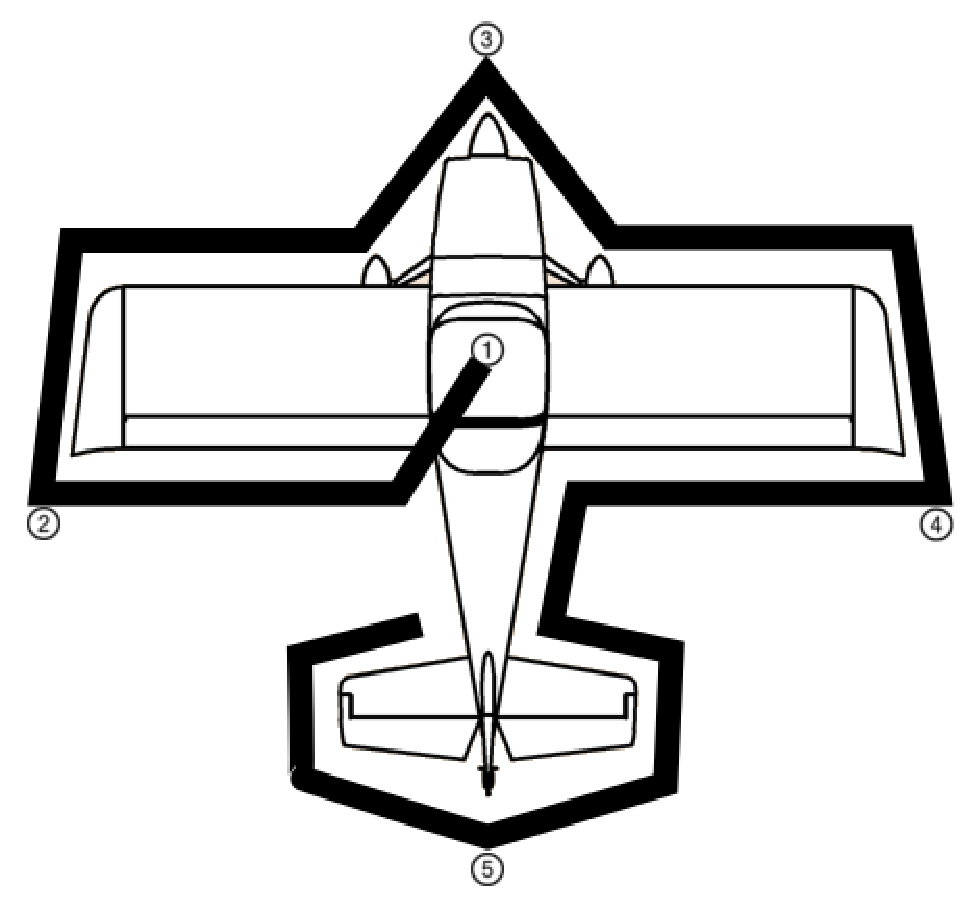
\includegraphics[height=0.5\textheight]{walkaround2.eps}
\caption{Walkaround}
\label{fig:walkaround}
\end{figure}

\section{Before Entering the Airplane}
%\begin{enumerate}[\circled{1}]
\circled{1}
\begin{enumerate}[(1)]
\item Master and EFIS -- ON
\item Fuel gauges -- CHECK
\item Flaps -- EXTEND FULLY
\item Master and EFIS -- OFF
\end{enumerate} 	
\circled{2}
\begin{enumerate}[(1)]
\item Left wing control surfaces -- CHECK
\item AoA port -- CLEAR
\item Pitot tube -- CLEAR
\item Left tank -- CHECK LEVEL and CAP SECURE
\item Left strainer -- DRAIN and CHECK
\item Left wheel -- CHECK
\end{enumerate}
\circled{3}
\begin{enumerate}[(1)]
\item Fuel vents -- CLEAR
\item Windshield -- CLEAN and SECURE
\item Air inlets -- CLEAR
\item Prop and Spinner -- CHECK
\item Oil -- Check level (~6 Qt)
\item Cowls -- SECURE
\end{enumerate}
\circled{4}
\begin{enumerate}[(1)]
\item Right tank -- CHECK LEVEL and CAP SECURE
\item Right strainer -- DRAIN and CHECK
\item Right wing control surfaces -- CHECK
\item Right wheel -- CHECK 
\end{enumerate}
\circled{5}
\begin{enumerate}[(1)]
\item Static port -- CLEAR
\item Rear Empennage Fairing -- CHECK
\item Elevator -- CHECK
\item Rudder -- CHECK
\item Tail wheel -- CHECK
\end{enumerate}

\section{Before Starting the Engine}
\begin{enumerate}[(1)]
  \item Seats and Seat Belts -- Adjust and Lock
  \item Alternate air -- OFF (Emergency use only)
  \item Brakes -- Test
  \item Avionics -- OFF
  \item Flaps -- RETRACT IN STAGES ($20^\circ, 10^\circ, 0^\circ)$
\end{enumerate}

\section{Priming the Engine (Cold Engines Only)}
\begin{enumerate}[(1)]
  \item Propellor -- FINE
  \item Fuel valve -- SELECT
  \item Master -- ON
  \item EFIS -- ON
  \item Fuel pump -- ON
  \item Throttle -- OPEN FULL
  \item Mixture -- ADVANCE TO FULL RICH (Until slow but steady fuel flow achieved for 3-5s)
  \item Throttle -- CLOSED
  \item Mixture -- IDLE CUT OFF
  \item Fuel pump -- OFF
\end{enumerate}

\section{Starting Engine (Cold)}
\begin{enumerate}[(1)]
  \item Prime -- AS REQUIRED
  \item Throttle -- OPEN 1/4 TRAVEL
  \item Ignition Switch -- START (release when engine starts)
  \item Mixture -- FULL RICH (slowly and smoothly)
  \item Throttle -- SET 1000 RPM
  \item Oil Pressure -- CHECK (stop if not green in 30s)
  \item Ammeter -- ON AND CHARGING
  \item Mixture -- LEAN (for taxi)
  \item Avionics -- ON 
\end{enumerate}

\section{Starting Engine (Hot)}
\begin{enumerate}
  \item Mixture -- FULL LEAN
  \item Throttle -- FULL OPEN
  \item Inition -- ON
  \item Ignition Switch -- START (release when engine starts)
  \item Mixture -- FULL RICH (slowly and smoothly)
  \item Throttle -- CLOSE AND SET 1000 RPM
  \item Ammeter -- ON AND CHARGING
  \item Mixture -- LEAN (for taxi)
  \item Avionics -- ON 
\end{enumerate}

\section{Ground Running and Warm-up}
\begin{enumerate}[(1)]
  \item Aircraft -- Into Wind
  \item Mixture -- RICH
  \item Propellor -- FINE
  \item Throttle -- SET 1000-1200 RPM (less than 2200 RPM on ground)
\end{enumerate} 

%\begin{center}
%NOTE

%Engine is warm enough when throttle can be opened without %faltering.
%\end{center}

\section{Power Check}
\begin{enumerate}[(1)]
  \item Brakes -- ON
  \item Fuel selector -- SWITCH
  \item Oil Temperature -- GREEN
  \item Oil Pressure -- GREEN
  \item Mixture -- RICH
  \item Throttle -- 1000 - 1500  RPM
  \item Propellor -- CYCLE x 3 (Avoid more than 500 RPM drop)
  \item Throttle -- SET 1800 RPM (50-65\% power)
  \item Magneto -- CHECK (175 drop 50 RPM difference)
  \item Alternate air -- Check for RPM drop on activation
  \item Engine instruments and Ammeter -- CHECK 
  \item Flights Instruments and Radios -- SET
  \item Beacon, Navigation lights -- ON (as required)
  \item Wing Flaps - CHECK 
\end{enumerate} 

\begin{center}
NOTE
 
Any ground check that requires full throttle operation must be limited to three minutes, or less if the cylinder head temperature should exceed the maximum as stated in this manual.
\end{center}

\section{Take Off}
\subsection{Normal Take Off}
\begin{enumerate}[(1)]
  \item Flaps -- UP
  \item Throttle -- OPEN 
  \item Mixture -- RICH (lean for field elevation)
  \item Rotate -- 70 KIAS
  \item Climb Speed -- $V_y$ 104 KIAS 
\end{enumerate}
\subsection{Maximum Performance Take Off}
\begin{enumerate}[(1)]
  \item Flaps -- 15$^{\circ}$
  \item Brakes -- APPLY
  \item Throttle -- FULL THROTTLE  
  \item Mixture -- RICH (lean for field elevation)
  \item Brakes -- RELEASE
  \item Rotate -- 55 KIAS
  \item Climb Speed -- $V_x$ 74 KIAS 
  \item Wing Flaps -- RETRACT after reaching 74 KIAS
\end{enumerate}
\begin{center}
NOTE

Do not reduce power until wing flaps have been retracted.
\end{center}

\section{Enroute Climb}
\begin{enumerate}[(1)]
  \item Airspeed -- $V_y$ 104 KIAS or higher
  \item Power -- 25 INCHES or FULL THROTTLE and 2500rpm 
  \item Mixture -- LEAN as required
\end{enumerate}

\section{Cruise}
\begin{enumerate}[(1)]
\item Power -- 15-25 INCHES, 2100 - 2500 RPM (no more than 75\%)
\subitem Performance (75\% Power): RPM 2450, Fuel Flow 12.3 Gal (47l/h) %~10gal 48 liters/h
\subitem Economy (65\% Power): RPM 2350, Fuel Flow 9.5 Gal (36l/h) %8.66 ~33l/h
\item Mixture -- LEAN as required
\end{enumerate}

\section{Before Landing}
\begin{enumerate}[(1)]
\item Mixture -- RICH
\item Propeller -- HIGH RPM
\item Airspeed -- 70-80 KIAS (flaps UP)
\item Wing Flaps -- As Required (20$^{\circ}$below 96 KIAS 20$^{\circ}$-40$^{\circ}$ below 87 KIAS)
\item Aisrpeed -- 60-70 KIAS (flaps DOWN)
\end{enumerate}

\section{Balked Landing (Go-around)}
\begin{enumerate}[(1)]
\item Power -- FULL THROTTLE and 2700rpm
\item Wing Flaps -- RETRACT to 20$^{\circ}$
\item Airspeed --  70 KIAS
\item Wing Flaps -- RETRACT slowly
\end{enumerate}

\section{Engine Shutdown}
\begin{enumerate}[(1)]
\item Propellor -- FINE 
\item Throttle  -- IDLE until CHT drop
\item Mixture  --  IDLE CUT OFF
\item Master -- OFF when engine stops
\end{enumerate}

\section{Amplified Procedures}
%\subsection{Power checks}

\subsection{Before starting engine}
When testing the brakes both brake pedals should have a similar feel and a firm resistance after 1/2" of pedal travel.

\subsection{Throttle operation}
Throttle movements from full power to idle or from idle to full power are full range movements. Full range throttle movements must be performed over a minimum time duration of 2 to 3 seconds. Performing a full range throttle movement at a rate of less than 2 seconds is considered a rapid or
instant movement. Performing rapid movements may result in detuned counterweights which may lead to failure of the counterweight lobes and subsequent engine damage.


\subsection{Take off}
The auxiliary fuel pump is normally off during take offs.  If there is evidence of fuel vapour or rough engine operation the pump should be turned on.

Full throttle runups over loose gravel are harmful to propeller tips.  Rolling take offs where the throttle is advance gently is suggested.  

Use full-rich mixture during takeoff or climb. Careful observation of engine temperature instruments should be practiced to ensure the limits specified are never exceeded.
Prior to take off from fields above 3000 ft elevation the mixture should be leaned.


\subsection{Wing flap settings}
Check that the flaps are retracted evenly. When flap is needed to shorten take off runs, no more than 15$^{\circ}$ is suggested.

\subsection{Enroute climb}
Normal climbs are performed with the flaps retracted and the airspeed 5 to 15 kt faster than best rate of climb speed.  Power selected should not be less than 25" MAP and 2500 rpm. Full throttle climb at 2400 RPM and higher is allowed. 

\subsection{Cruise}
Normal cruising is perfromed between 55\% and 75\% power.  
For reduced noise levels the lowest RPM in the green arc for the desired power setting is suggested.

For maximum service life, maintain the following limits are recommended for continuous cruise operation:\\
\begin{itemize}
\item Engine power setting - 65\% of rated or less.
\item Cylinder head temperatures - 400$^{\circ}$F or below.
\item Oil temperature 165$^{\circ}$F to 220$^{\circ}$F.
\end{itemize}
\begin{center}
NOTE\\

After engine rework cruising should be done at 65\% to 75\% power for 50 hours or until oil consumption stabilise.
\end{center}

\subsection{Mixture leaning in flight}
The relationship between Mixture setting and engine power is indicated in Figure~\ref{fig:Leaning_graph}.

\begin{figure}[H]
\centering
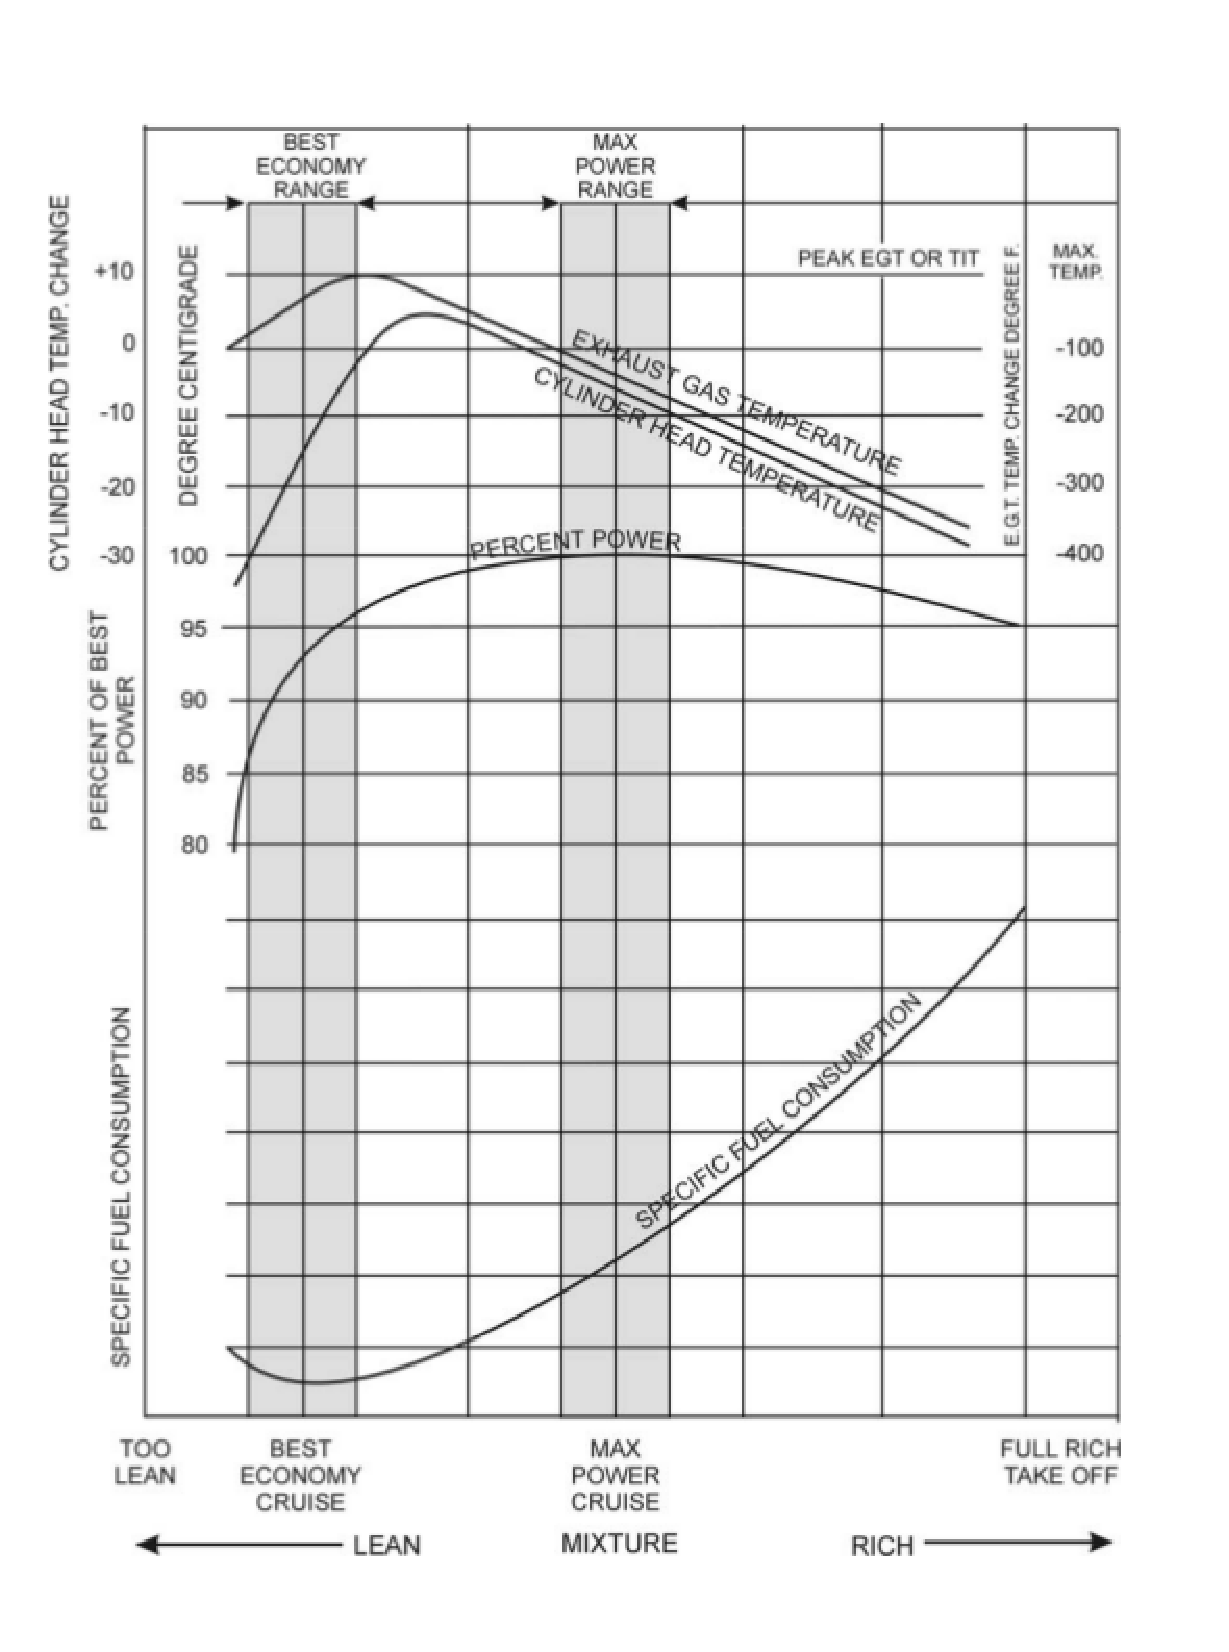
\includegraphics[height=0.8\textheight]{Leaning_graph.eps}
\caption{Lycoming power leaning curve}
\label{fig:Leaning_graph}
\end{figure}

\subsection{Leaning with Exhaust Gas Temperature (EGT) Gauge}
\subsubsection{Maximum Power Cruise}
\begin{enumerate}[(1)]
\item Approximately 75\% Power.
\item Never lean beyond 150$^{\circ}$ on RICH side of peak EGT.
\item Monitor cylinder head temperatures.
\end{enumerate}

\subsubsection{Best Economy Cruise}
\begin{enumerate}[(1)]
\item Approximately 75\% Power and BELOW.
\item Operate at PEAK EGT.
\end{enumerate}

\subsection{Leaning with Manual Mixture Control}
Economy cruise, 75\% power or less, without flowmeter or EGT guage
\begin{enumerate}[(1)]
\item Slowly move mixture control from FULL RICH position toward lean posittion.
\item Continue leaning until slight loss of power is noted\\ (loss of power may or may not be accompanied by roughness.)
\item Enrich until engine runs moothly and power is regained.
\end{enumerate}

\subsection{Let down}
Sudden cooling is detrimental to the good health of the aircraft engine. Lycoming Service Instruction 1094D recommends a maximum temperature change of 50${^\circ}$F per minute to avoid shock cooling of the cylinders.

Pilots must avoid fast letdowns with very low power (high-cruise RPM and low manifold pressure), along with rich mixtures that contribute to sudden cooling. It is recommended that pilots maintain at least 15" MAP or higher, and set the RPM at the lowest cruise position. 

Letdown speed should not exceed high cruise speed or approximately 1,000 feet per minute of descent. Keeping descent and airspeed within these limits will help to prevent the sudden cooling that may result in cracked cylinder heads, warped exhaust valves, and bent pushrods.

The mixture setting also has an effect on engine cooling. To reduce spark plug fouling and keep the cylinder cooling within the recommended 50${^\circ}$F per-minute limit, the mixture should be left at the lean setting used for cruise and then richened gradually during the descent from altitude. The lean mixture, maintaining some power and using a sensible airspeed should achieve the most efficient engine temperatures possible.

\subsection{Crosswind Landing }
When landing in a crosswind, use the minimum flap setting required for the field length available.

\subsection{Go-around }
In a go-aroud, apply full throttle and 2700 RPM smoothly using fine pitch.  Reduce wing flaps promptly to climb setting.   Upon reaching a safe airspeed with positive rate of climb flaps should be retracted fully.

\subsection{Cold Weather Operation}
Prior to starting in cold temperatures it is advisable to pull the propeller through several times.  

\begin{center}
NOTE\\

When pulling through the propeller treat it as if the ignition is on.  A loose or broken ground wire to either magento could cause the engine to fire.
\end{center}

\section{Aerobatic Flight}
\subsection{Aerobatic Flight}
The aircraft is capable of easily performing basic aerobatic manoeuvres. This capability is due to its relatively high power loading and aerodynamic cleanliness which produces the speed or energy needed.  Excessive speed build-up can occur very quickly and should be of primary concern when attempting and practicing aerobatics.  Elevator stick forces are relatively light, over stressing could easily occur.  Pilots should received formal aerobatic training before attempting aerobatic flight.

\subsection{Airspeed Aerobatic Manoeuvres}
The aircraft is capable of performing the aerobatic manoeuvres listed in Table~\ref{tab:aero_speeds}.

\begin{table}[h]
\caption{Aerobatic Entry Speeds}
\label{tab:aero_speeds}
  \begin{tabularx}{\linewidth}{|
    >{\hsize=0.6\hsize}X|
    >{\hsize=0.2\hsize}X|
    >{\hsize=0.2\hsize}X|
  }
\hline
Manoeuvre: & Speed \newline Minimum & Speed \newline Maximum\\
\hline
Loops, Horizontal eights:&122 kt &  165 kt\\
\hline
Immelman Turns: & 130 kt& 165 kt\\
\hline
Aileron Rolls, Barrel Rolls: &104 kt& 165 kt\\
\hline
Snap rolls &70 kt& 96 kt\\ 
\hline
Vertical Rolls: & 156 kt & 165 kt\\
\hline
Split-S:       & 87 kt&  96 kt\\
\hline
\end{tabularx}
\end{table}

 

\chapter{Performance}
\thispagestyle{fancy}
\minitoc[n] % Creating an actual minitoc

\section{Introduction}
Performance data charts on the following pages are presented in order to know what to expect from the aircraft under various conditions.  Values in this section are factory numbers and must be verified on your aircraft.

\section{Use of Performance Information}
The performance information should allow the pilot to plan all stages of a flight including take off, climb out, cruise and landing.  Particular attention should be paid to fuel required and monitored against fuel used during actual flight conditions.

\section{Stall speeds}
Stall speeds are presented for 0$^{\circ}$ angle of bank only.  Stall speeds increase with increasing angle of bank.

\begin{table}[h]
\caption{Stall speeds}
\label{tab:stall speeds}
  \begin{tabularx}{\linewidth}{
    |>{\hsize=0.2\hsize}X| 
     >{\hsize=0.6\hsize}X|
     >{\hsize=0.2\hsize}X| 
} 
 \hline
 Weight & Flap Deflection &  Airspeed\\ 
 \hline
 1800 lbs & UP  & 56 kt \\ 
 \hline
 1800 lbs & 40$^{\circ}$ & 51 kt\\ 
 \hline
\end{tabularx}
\end{table}

\section{Takeoff Distance}
Takeoff distance given below are in standard conditions and optimum pilot technique.

\begin{table}[h]
\caption{Takeoff Distance}
\label{tab:to_distance}
  \begin{tabularx}{\linewidth}{
    |>{\hsize=0.2\hsize}X| 
     >{\hsize=0.6\hsize}X|
     >{\hsize=0.2\hsize}X| 
} 
 \hline
 Description & Weight &  Distance\\ 
 \hline
 Solo Weight  & 1400 lbs  & 250 ft \\ 
 \hline
 Gross Weight  & 1800 lbs & 500 ft\\ 
 \hline
 \end{tabularx}
\end{table}

\section{Landing Distance}	
Landing distance given below are in standard conditions and optimum pilot technique.

\begin{table}[h]
\caption{Landing Distance}
\label{tab:landing_dist}
  \begin{tabularx}{\linewidth}{
    |>{\hsize=0.2\hsize}X| 
     >{\hsize=0.6\hsize}X|
     >{\hsize=0.2\hsize}X| 
} 
 \hline
 Description & Weight &  Distance\\ 
 \hline
 Solo Weight  & 1400 lbs  & 350 ft \\ 
 \hline
 Gross Weight  & 1800 lbs & 500 ft\\ 
 \hline
\end{tabularx}
\end{table}

\section{Rate of Climb}
Rate of Climb values given below are in standard conditions and optimum pilot technique.

\begin{table}[h]
\caption{Rate of Climb}
\label{tab:roc}
  \begin{tabularx}{\linewidth}{
    |>{\hsize=0.2\hsize}X| 
     >{\hsize=0.6\hsize}X|
     >{\hsize=0.2\hsize}X| 
} 
 \hline
 Description & Weight &  Rate\\ 
 \hline
 Solo Weight  & 1400 lbs  & 2550 fpm \\ 
 \hline
 Gross Weight  & 1800 lbs & 1900 fpm\\ 
 \hline
\end{tabularx}
\end{table}

\section{Range Profile}
Range profile for different power settings at a typical cruise pressure altitude of 8000 ft is given below.

\begin{table}[h]
\caption{Range Profile}
\label{tab:range}
\begin{tabularx}{\linewidth}{
    |>{\hsize=0.2\hsize}X| 
     >{\hsize=0.6\hsize}X|
     >{\hsize=0.2\hsize}X| 
    }
\hline 	
Setting & Altitude & Range \\
\hline
75\% Power	& Pressure Altitude 8000 ft &\textit{664 nm}\\
\hline
55\% Power 	& Pressure Altitude 8000 ft &\textit{812 nm}\\
\hline 
\end{tabularx}
\end{table}

The fuel consumption for either best power or best economy settings are provided in the engine operating manual and reproduced in Figure~\ref{fig:fuelflow}.  

\begin{figure}[H]
\centering
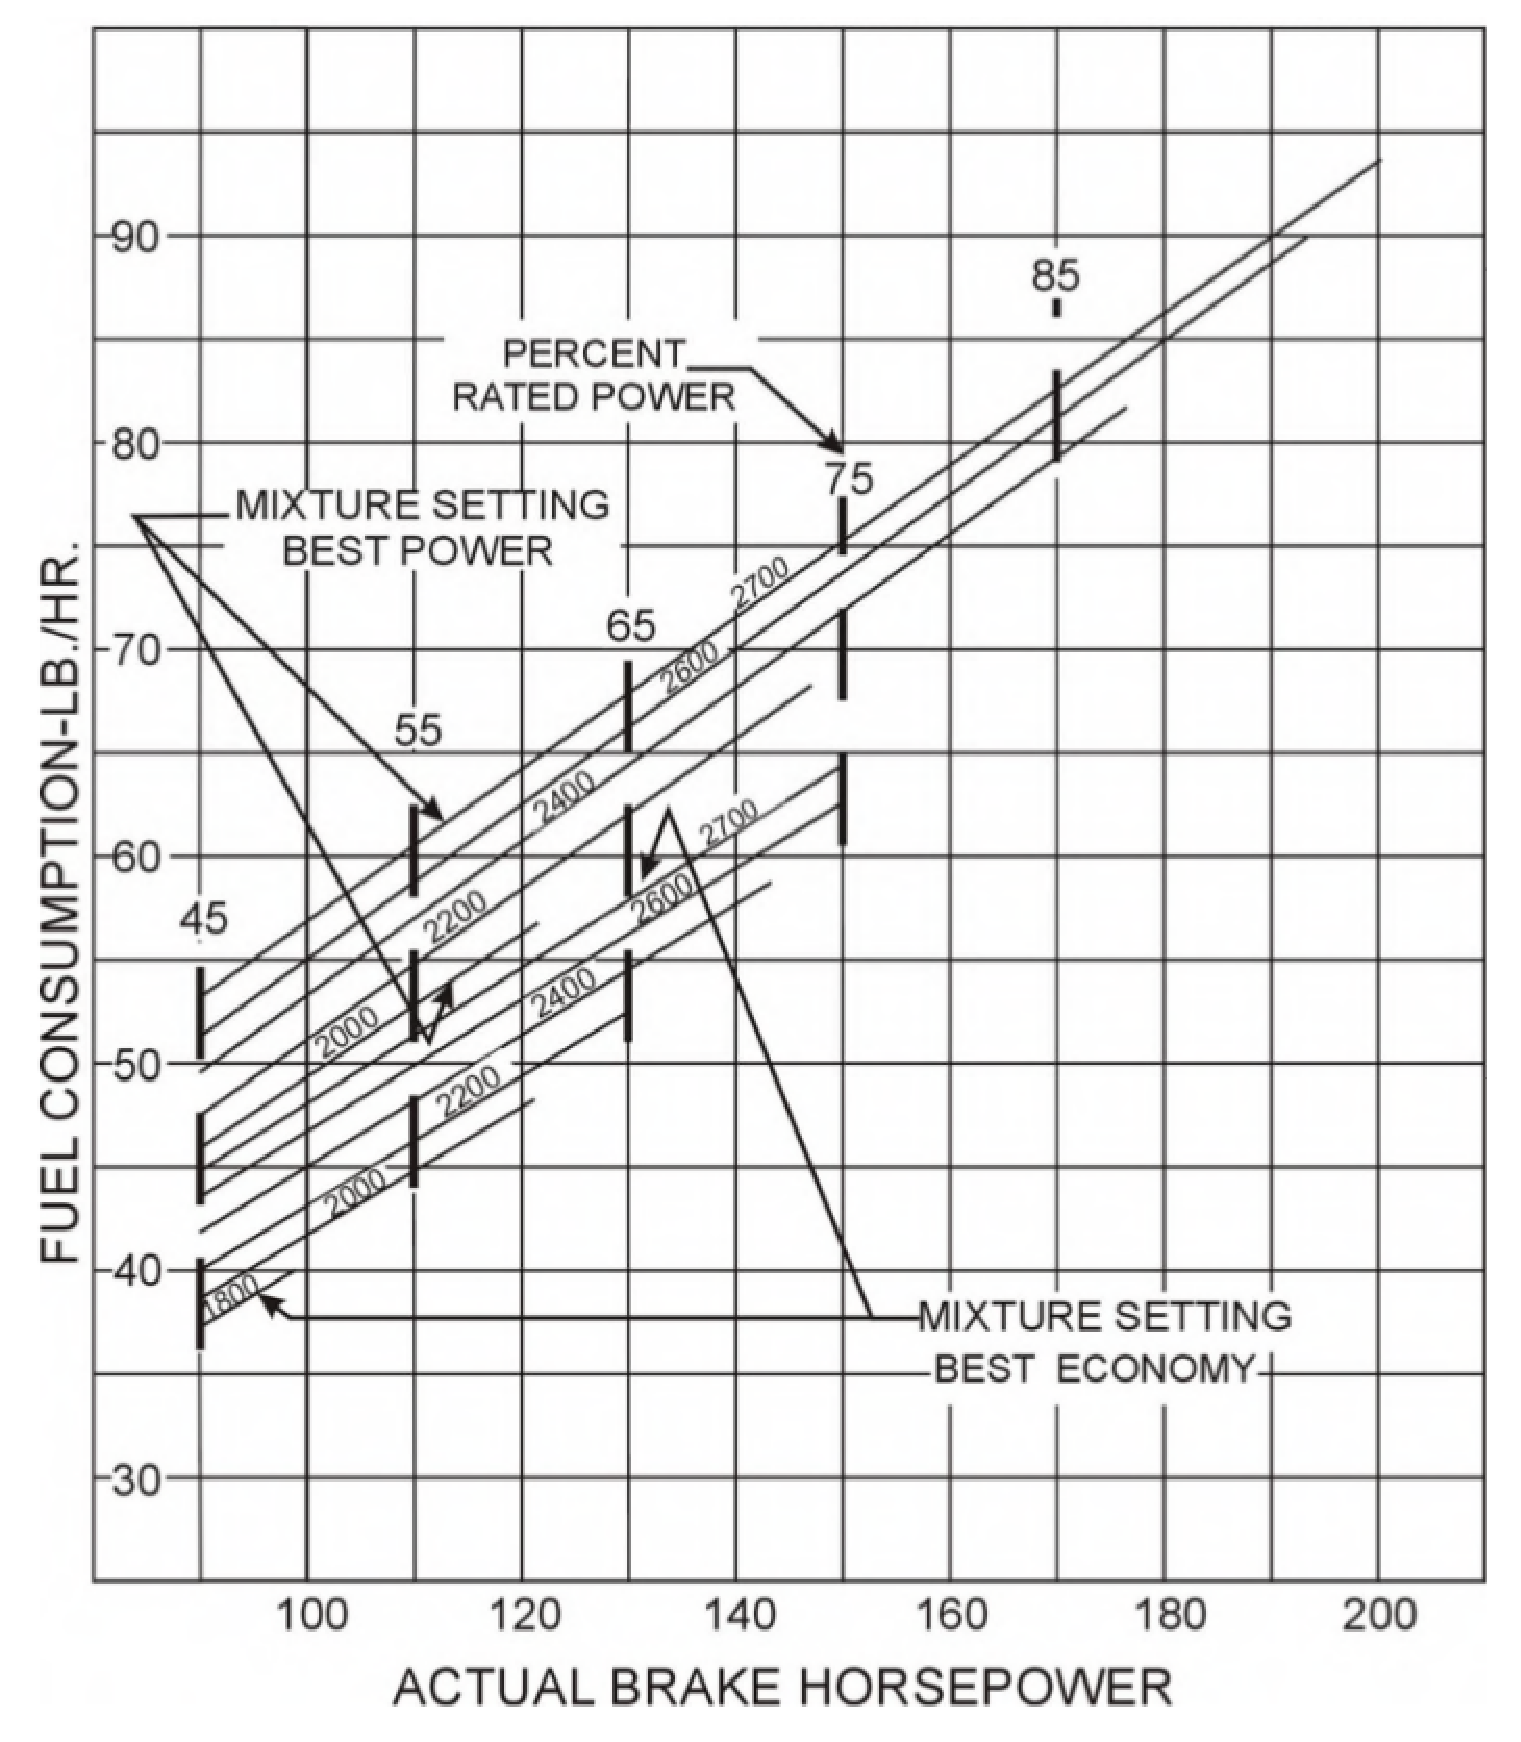
\includegraphics[height=0.75\textheight]{IO360-A1B6.eps}
\caption{Fuel consumption for Best Power and Best Economy setting. See the IO360 operators manual (Lycoming part no 60297-12) pg 52.}
\label{fig:fuelflow}
\end{figure}


\section{Cruise performance}
Cruise performance values given below is based on engine power settings alone.  Actual power 
settings depends on environment and altitude of operation. For detailed power settings, please
see Figure \ref{fig:engineperf}.
\begin{table}[h]
\caption{Operating conditions}
\label{tab:performance}
  \begin{tabularx}{\linewidth}{
    |>{\hsize=0.4\hsize}X| 
     >{\hsize=0.2\hsize}X|
     >{\hsize=0.2\hsize}X| 
     >{\hsize=0.2\hsize}X| 
} 
\hline
& RPM & Fuel Flow Gal/Hr. & Oil Use \newline Qts./Hr. \\
\hline
Normal Rated \newline 200 HP & 2700 & 15.4(58.3$\ell$/h) &.89 \\
\hline
Performance Cruise \newline  (75\% Rated) 150 HP & 2450 (23")&  12.3 (47$\ell$/h)  & .50 \\
\hline
Economy Cruise \newline (65\% Rated) 130 HP &  2350 (21") &  9.5 (36 $\ell$/h)&.44 \\
\hline
\end{tabularx}
\end{table}

\begin{figure}[tbh]
  \centering
  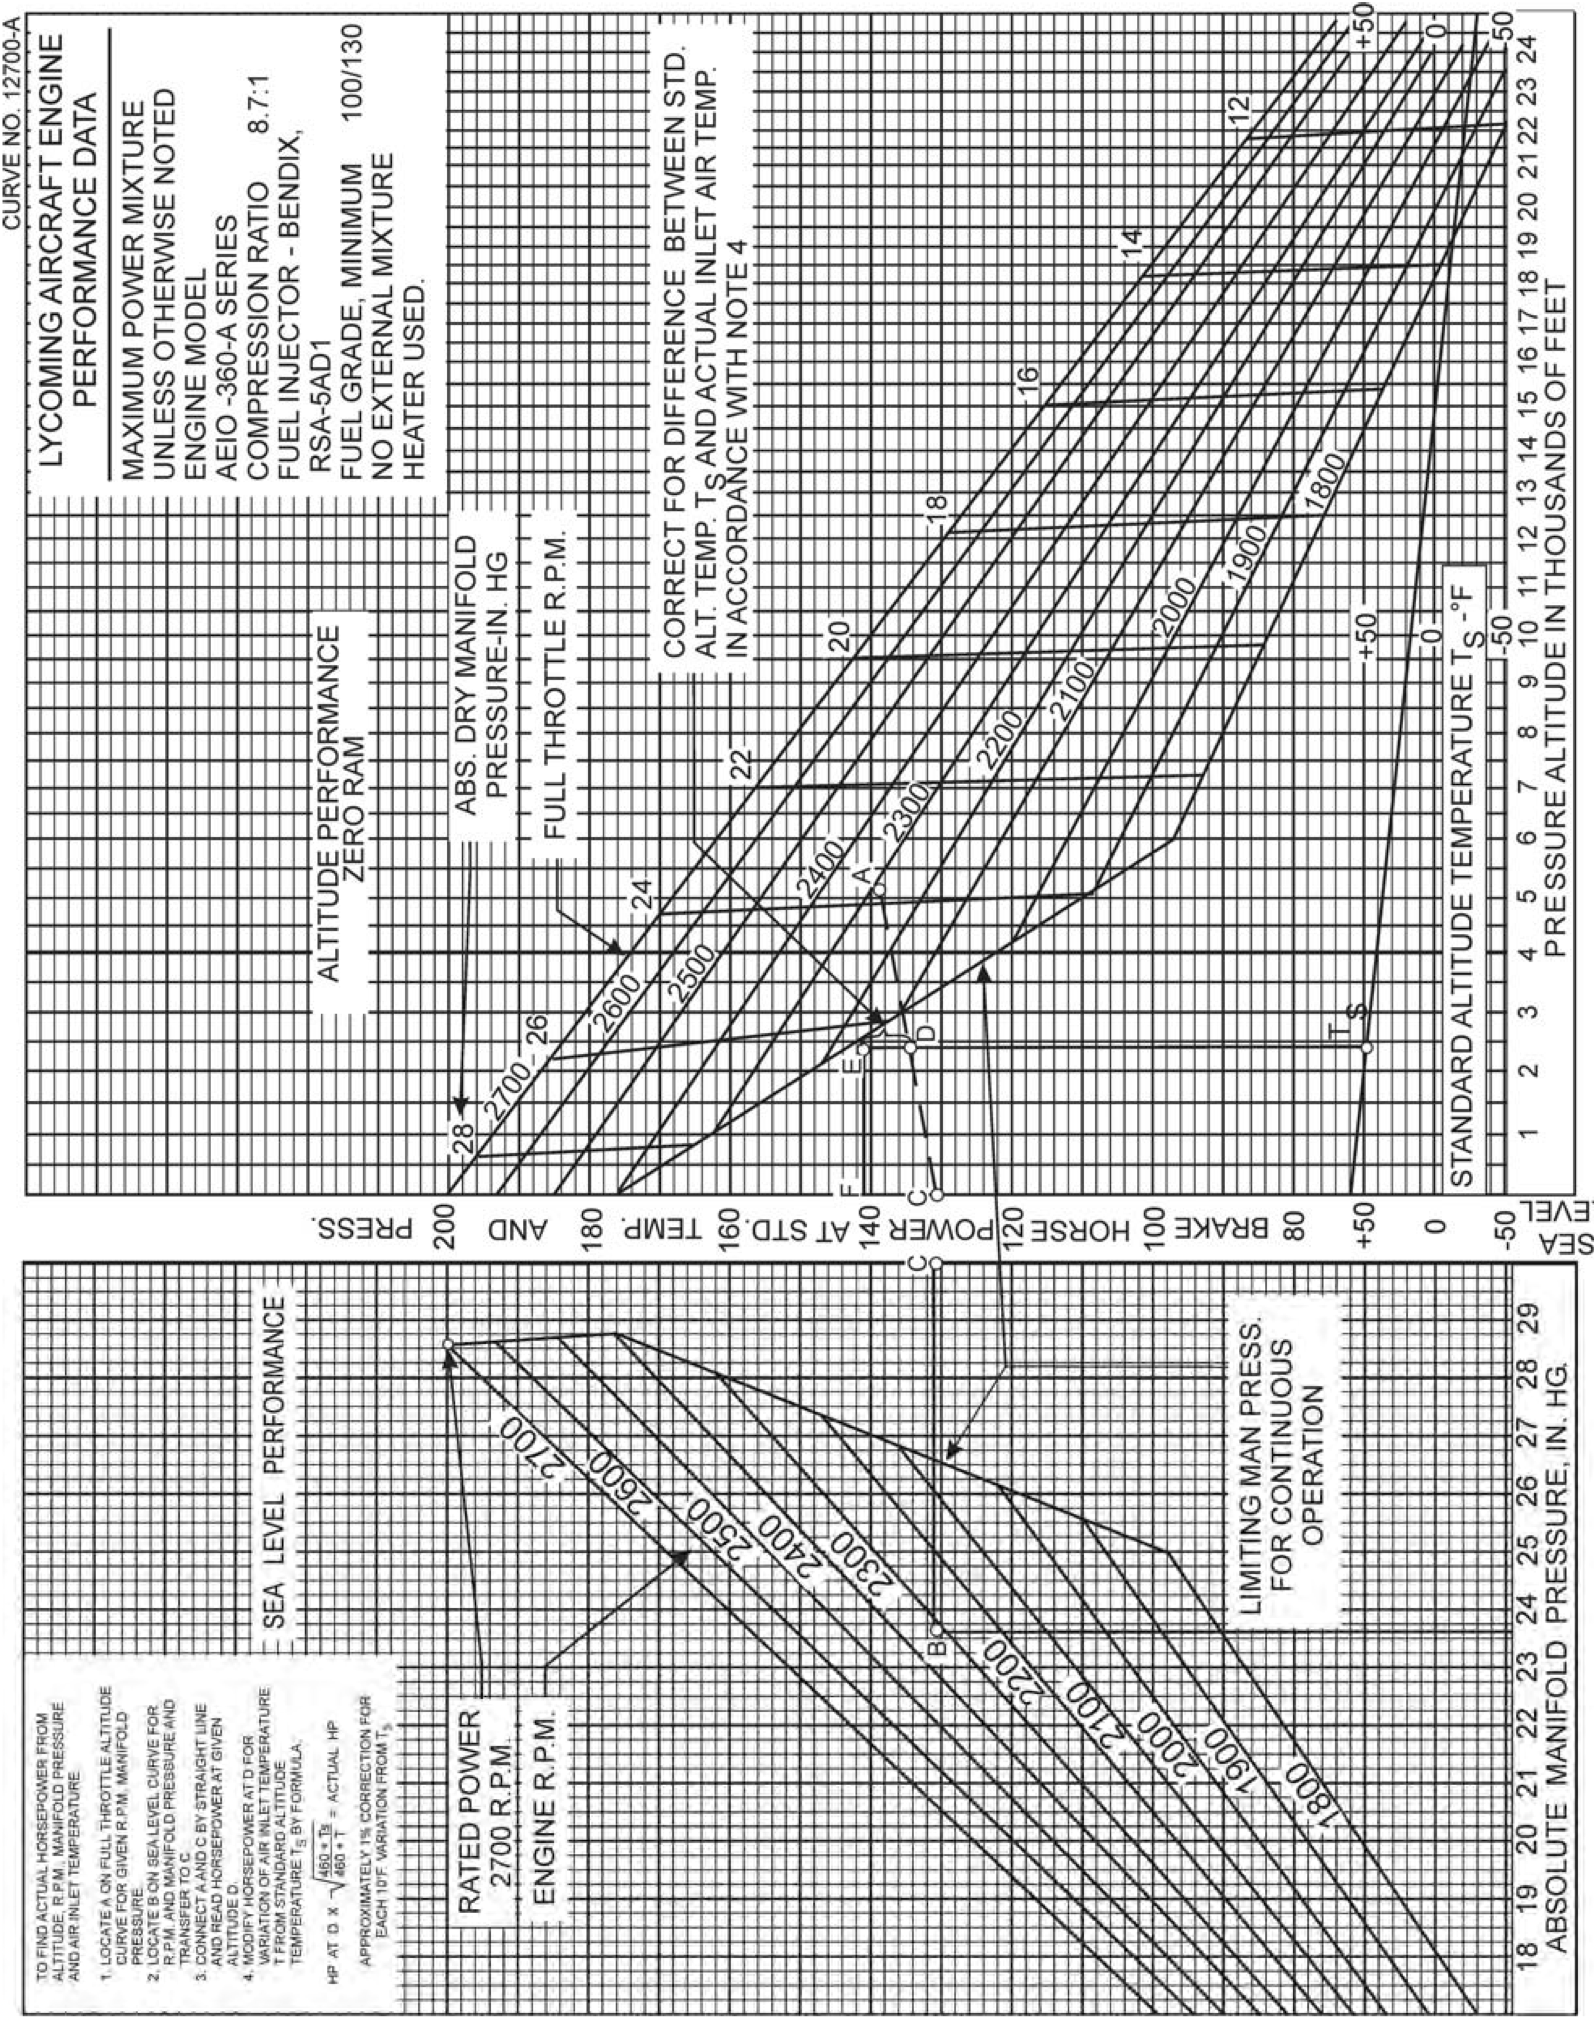
\includegraphics[height=0.9\textheight]{power-settings.png}
  \caption{Engine performance chart from the IO360 operators manual (Lycoming part no 60297-12) pg 68.}
  \label{fig:engineperf}
\end{figure}


\chapter{Weight and Balance}
\thispagestyle{fancy}
\minitoc[n] % Creating an actual minitoc

\section{Introduction}
This section describes the procedure for establishing the basic empty weight and moment of the airplane.  

It should be noted that specific information regarding the weight, arm, moment and installed equipment list for this airplane can only be found in the appropriate weight and balance records.

\section{Airplane weighing procedures}
The airplane should be weighed in the empty condition and in a level attitude.  Scales should be placed simultaneously under both main wheels and the tail wheel as shown in Figure~\ref{fig:wandb}.
\begin{figure}[h]
\centering
\includegraphics[width=1\textwidth]{wandb.eps}
\caption{Aircraft weighing orientation}
\label{fig:wandb}
\end{figure}

\subsection{Preparation}
Inflate tyres to recommended operating pressures.  Drain all fuel.  Drain all engine oil.  Move all seats to the most forward position.  Raise flaps to fully retracted position.  Place all control surfaces in neutral position.  
\subsection{Levelling}
Place scales under each wheel.  Level attitude is established at the datum line which is the cockpit rails.  
\subsection{Weighing}
With the airplane level, record the weight shown on each scale.  
\subsection{Measuring}
To keep all moments positive, a datum has been selected at a point forward of the prop spinner.  This point is 70 inches in front of the wing leading edge.  Measure the distance from both the main wheels to the aircraft datum.  Measure the distance from the tail wheel to the aircraft datum.
\subsection{Calculation}
Calculate the moment for both main wheels and the tail wheel by multiplying the distance to the datum with the measured weight for each.  Sum all the Moments and the Weights.  To obtain the empty Centre of Gravity divide the total moment by the total weight. 


\section{Weight and Balance}
The following information will enable the pilot to operate within the prescibed weight and center of gravity limitations.  

\subsection{Centre of Gravity limits}
The maximum weight and Centre of Gravity limits for both the Aerobatic and Normal Category operations are summarised in Table~\ref{tab:cofg_limits}.
\begin{table}[H]
\caption{Centre of gravity limits}
\label{tab:cofg_limits}
  \begin{tabularx}{\linewidth}{
    |>{\hsize=0.4\hsize}X| 
     >{\hsize=0.2\hsize}X|
     >{\hsize=0.2\hsize}X| 
     >{\hsize=0.2\hsize}X|
  }
%  \begin{tabular}{ |p{1in}|p{1in}|p{3.5in}| } 
 \hline
  Category & Weight \newline Maximum & C of G \newline Minimum & C of G \newline Maximum \\ 
   \hline
  Aerobatic & 1600 & 78.7" & 84.5"  \\ 
   \hline
  Normal    & 1800 & 78.7" & 86.8"  \\ 
 \hline
 \end{tabularx}
\end{table}

\subsection{Sample loading problems}
The following example in Table~\ref{tab:gross} shows the aircraft loaded to the maximum weight of 1800 lbs.  This is achieved by loading full fuel and 85lbs of the full 100 lbs baggage allowance.  A standard 170 lbs pilot and 170 lbs passenger occupy the seats.

\begin{table}[H]
\caption{Gross weight Sample loading problem}
\label{tab:gross}
  \begin{tabularx}{\linewidth}{
    |>{\hsize=0.4\hsize}X| 
     >{\hsize=0.2\hsize}X|
     >{\hsize=0.2\hsize}X| 
     >{\hsize=0.2\hsize}X| 
  }
%  \begin{tabular}{ |p{1in}|p{1in}|p{3.5in}| } 
 \hline
  Item & Weight [lbs]& Arm [inch] & Moment \newline [inch-.lbs] \\ 
 \hline
 Aircraft & 1122 & 79.14 & 88799.05 \\ 
 \hline
 Fuel (42Us Gal) & 252 & 80 & 20160.00 \\ 
 \hline
 Pilot & 170 & 97.48 & 16571.60 \\ 
 \hline
 Passenger & 170 & 97.48 & 16571.60 \\ 
 \hline
 Baggage (100 lbs max) & 85 & 126.78 & 10766.30 \\ 
 \hline
 Total (1800 lbs)& 1799 & 85.45 & 152878.55 \\ 
 \hline
\end{tabularx}
\end{table}

The second example in Table~\ref{tab:aerobatic} shows the aircraft loaded within the aerobatic limits.  The same standard 170 lbs pilot and his 170 lbs passenger can only take half tanks and little or no baggage.

\begin{table}[H]
\caption{Aerobatic weight Sample loading problem}
\label{tab:aerobatic}
  \begin{tabularx}{\linewidth}{
    |>{\hsize=0.4\hsize}X| 
     >{\hsize=0.2\hsize}X|
     >{\hsize=0.2\hsize}X| 
     >{\hsize=0.2\hsize}X| 
  }
%  \begin{tabular}{ |p{1in}|p{1in}|p{3.5in}| } 
 \hline
  Item & Weight [lbs]& Arm [inch] & Moment \newline [inch-.lbs] \\ 
 \hline
 Aircraft & 1122 & 79.14 & 88799.05 \\ 
 \hline
 Fuel (21 Us Gal) & 126 & 80 & 10080.00 \\ 
 \hline
 Pilot & 170 & 97.48 & 16571.60 \\ 
 \hline
 Passenger & 170 & 97.48 & 16571.60 \\ 
 \hline
 Baggage (100 lbs) & --- & 126.78 & --- \\ 
 \hline
 Total (1800 lbs)& 1588 & 83.14 & 132022.25 \\ 
 \hline
\end{tabularx}
\end{table}

Figure ~\ref{fig:coglimits} shows the centre of gravity limits plotted graphically.  The Normal category operation envelope is plotted with a solid blue line.  The Aerobatic operation envelope is plotted with a dashed blue line.  The gross weight sample is plotted as a solid dot and the aerobatic weight sample is plotted as a plus sign.

\begin{figure}[H]
\centering
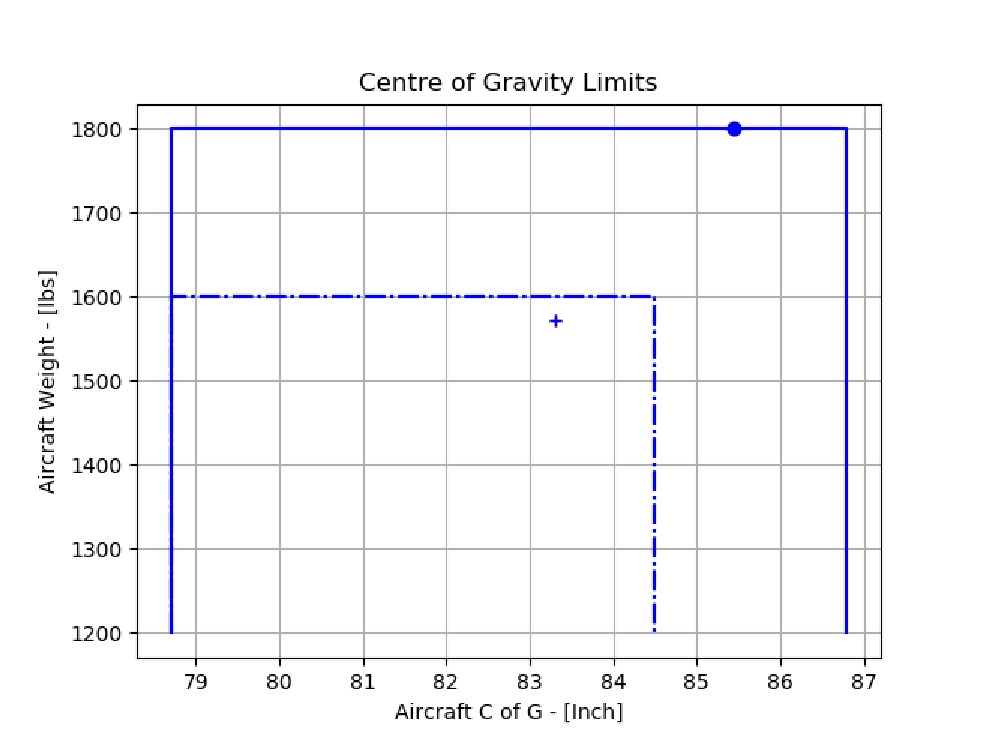
\includegraphics[width=1\textwidth]{coglimits.eps}
\caption{Aircraft weighing orientation}
\label{fig:coglimits}
\end{figure}

A blank table is provided in Table~\ref{tab:worksheet} to calculate the specific weight and balance for your aircraft.

\begin{table}[H]
\caption{Weight and Balance worksheet}
\label{tab:worksheet}
  \begin{tabularx}{\linewidth}{
    |>{\hsize=0.4\hsize}X| 
     >{\hsize=0.2\hsize}X|
     >{\hsize=0.2\hsize}X| 
     >{\hsize=0.2\hsize}X| 
  }
 \hline
  Item & Weight [lbs]& Arm [inch] & Moment \newline [inch-.lbs] \\ 
 \hline
 Aircraft & 1122 & 79.14 & 88799.05 \\ 
 \hline
 Fuel (42Us Gal) & ... & 80 &... \\ 
 \hline
 Pilot & ... & 97.48 &... \\ 
 \hline
 Passenger & ... & 97.48 &... \\ 
 \hline
 Baggage (100 lbs) & ... & 126.78 &... \\ 
 \hline
 Total (1800 lbs)& ... & ...&... \\ 
 \hline
\end{tabularx}
\end{table}


\chapter{Systems}
\thispagestyle{fancy}
\minitoc[n] % Creating an actual minitoc

\section{Introduction}


\section{Airframe}
The airframe is aluminium alloy construction except for steel components comprising the engine mount, main
landing gear mounts, control bellcranks and other miscellaneous items. Fibreglass mouldings are used for the
tips of wings and tail surface as well as for the engine cowls, wheel spats and empennage fairings.
The aircraft is conventionally configured with a non laminar flow aerofoil; the effect of surface irregularities is
relatively minor compared to a laminar flow aerofoil.

\section{Engine and propeller}
The aircraft is powered by a LYCOMING IO-360-A1B6 four cylinder, direct drive, horizontally opposed, air cooled, fuel injected engine rated at 200 HP at 2700 rpm. 

The engine is fitted with a 60-amp 14-volt alternator,
Sky Tec starter, high-pressure fuel pump and dual magneto ignition system. 

The induction air filter is mounted in
a ram air snorkel in the left air intake. An alternate air door is mounted to the side of the air snorkel for emergency
use should the induction intake or filter be blocked.

The exhaust system is all-stainless Vetterman four into two configuration and no mufflers. A heat shroud provides cabin
heat as required being ducted to the centre section of the firewall.

Please refer to the Lycoming Operators Handbook for detailed information on maintenance, care and operation
of the engine.

\section{Landing gear}
In conventional configuration the landing gear legs are of spring steel (6150).%, to which a preformed stiffener has been fitted to the front of main legs to improve dampening. 
The tail wheel is steerable and additional steering is possible through differential braking.

The main gear wheels are fitted with Cleveland wheels and disc brakes. The braking system consists of toe
brakes attached to the rudder pedals operating individual Cleveland brake cylinders to each of the main landing
wheels.
These share a common reservoir installed on the top right front face of the fire wall. The brake fluid used is MIL-
H-5606 and is red in colour.

Tyres and synthetic tubes are used.  The tyres are 6-ply and 5.00x5 in size.  Typical tyre pressure of 2.4 bar or 35 psi is used.

\section{Flying controls}
Flight control integrity is essential for safe flight. At installation or after maintenance it should be confirmed that
ALL controls are connected, secured and safe tied and that they all operate within the specified ranges
smoothly and in the correct direction. Full travel should be confirmed prior to each flight. NO play should be
permitted in the control hinges; sloppiness may induce flutter. Similarly trim tabs must be free of play.

Dual controls are provided. Elevator and Ailerons are operated through a system of adjustable pushrods. The
rudder is operated through a cable system to the rudder pedals. 

An electric elevator and aileron trim system
enables operation of the elevator trim tab and aileron spring bias system.
The elevator and aileron trims can be operated from a rocker switch on the instrument panel. 

\section{Engine controls}
Engine controls consist of a throttle control, pitch control, mixture control,
cabin heat and an alternate air control, mounted at centre beneath the avionics panel.

The throttle (black) is used to adjust engine power output, forward being full throttle and rearward for idle. A
throttle friction nut is located at the base of the control.

The propeller pitch control (blue) is located between the throttle and mixture control. Forward is full fine and
rearwards coarse. The control is of the vernier type and can be operated by rotating the blue knob clockwise or
anti clockwise for small adjustments or by pressing the centre knob in and pushing or pulling the control in or
out.

The mixture control (red) is used to adjust the fuel to air ratio. The engine is shut down by placing the mixture
control in the idle cut-off, or rearward position. The control is of the vernier type and can be operated by rotating
the red knob clockwise or anti clockwise for small adjustments or by pressing the centre knob in and pushing or
pulling the control in or out.

%The cabin heat is used to operate a door on the exhaust heat shroud . To activate, the ratchet cable and knob must be pulled to open the hot air inlet.

The alternate air is used to operate a sliding door on the side of the induction box. To activate, the ratchet cable
and knob must be pulled to open the door. This allows the engine to obtain warm unfiltered air from within the
cowling area. This control should only be used when an induction filter or intake blockage is suspected. Once
operated the control should be manually reset following rectification of the induction system blockage.

\section{Fuel System}
Fuel is stored in two 21 US gal (20 US gal usable) tanks secured to the leading edge structure with screws and
plate nuts. Fuel drains are fitted to the lowest point of each tank (and of the fuel system) and should be drained
prior to the first flight of the day to check for sediment and water.

Two fuel tank vents are located under the main fuselage on the left and rights side just forward of the main
landing gear attachments. These should be checked for any blockages.

The fuel selector valve is located in the centre column. It has four selectable positions - left or right tank and two
fuel shut-off positions.

An auxiliary electric fuel boost pump is fitted forward of the fuel selector on the cabin side of the fire wall and is
used in case of engine driven pump failure and is also used %during take off and landing, and 
when changing fuel
tanks in flight. A switch marked FUEL PUMP is located on the instrument panel.

%An airframe fuel filter is located in the gascolator on the right side of the engine firewall. This filter element
%should be inspected at least every 100hrs or Annual whichever comes first. Shorter cleaning intervals should be
%adopted should fuel quality be questionable.
Two fuel quantity indicators form part of the EFIS display and receive a signal from capacitive type fuel
probes mounted in the fuel tanks. Both are marked to indicate the appropriate fuel tank. These indicators only
register from a set quantity and NOT from full. As with all fuel gauges, these will tend to be inaccurate
when flight attitude is not coordinated or level and during turbulence.

A FUEL FLOW indicator and TOTAL FUEL QTY readout form part of the EFIS display and obtains fuel flow information
from a sender unit mounted in the main fuel line between the fuel selector and the engine driven fuel pump. This
should be used as a more accurate way of determining fuel consumption and fuel remaining. This system relies
on the pilot accurately loading the current fuel quantity into the EFIS whenever fuel is added.

\section{Electrical System}
A block diagram of the aircraft electrical system is provided in Figure~\ref{fig:electrical}.

\begin{sidewaysfigure}
\begin{figure}[H]
\centering
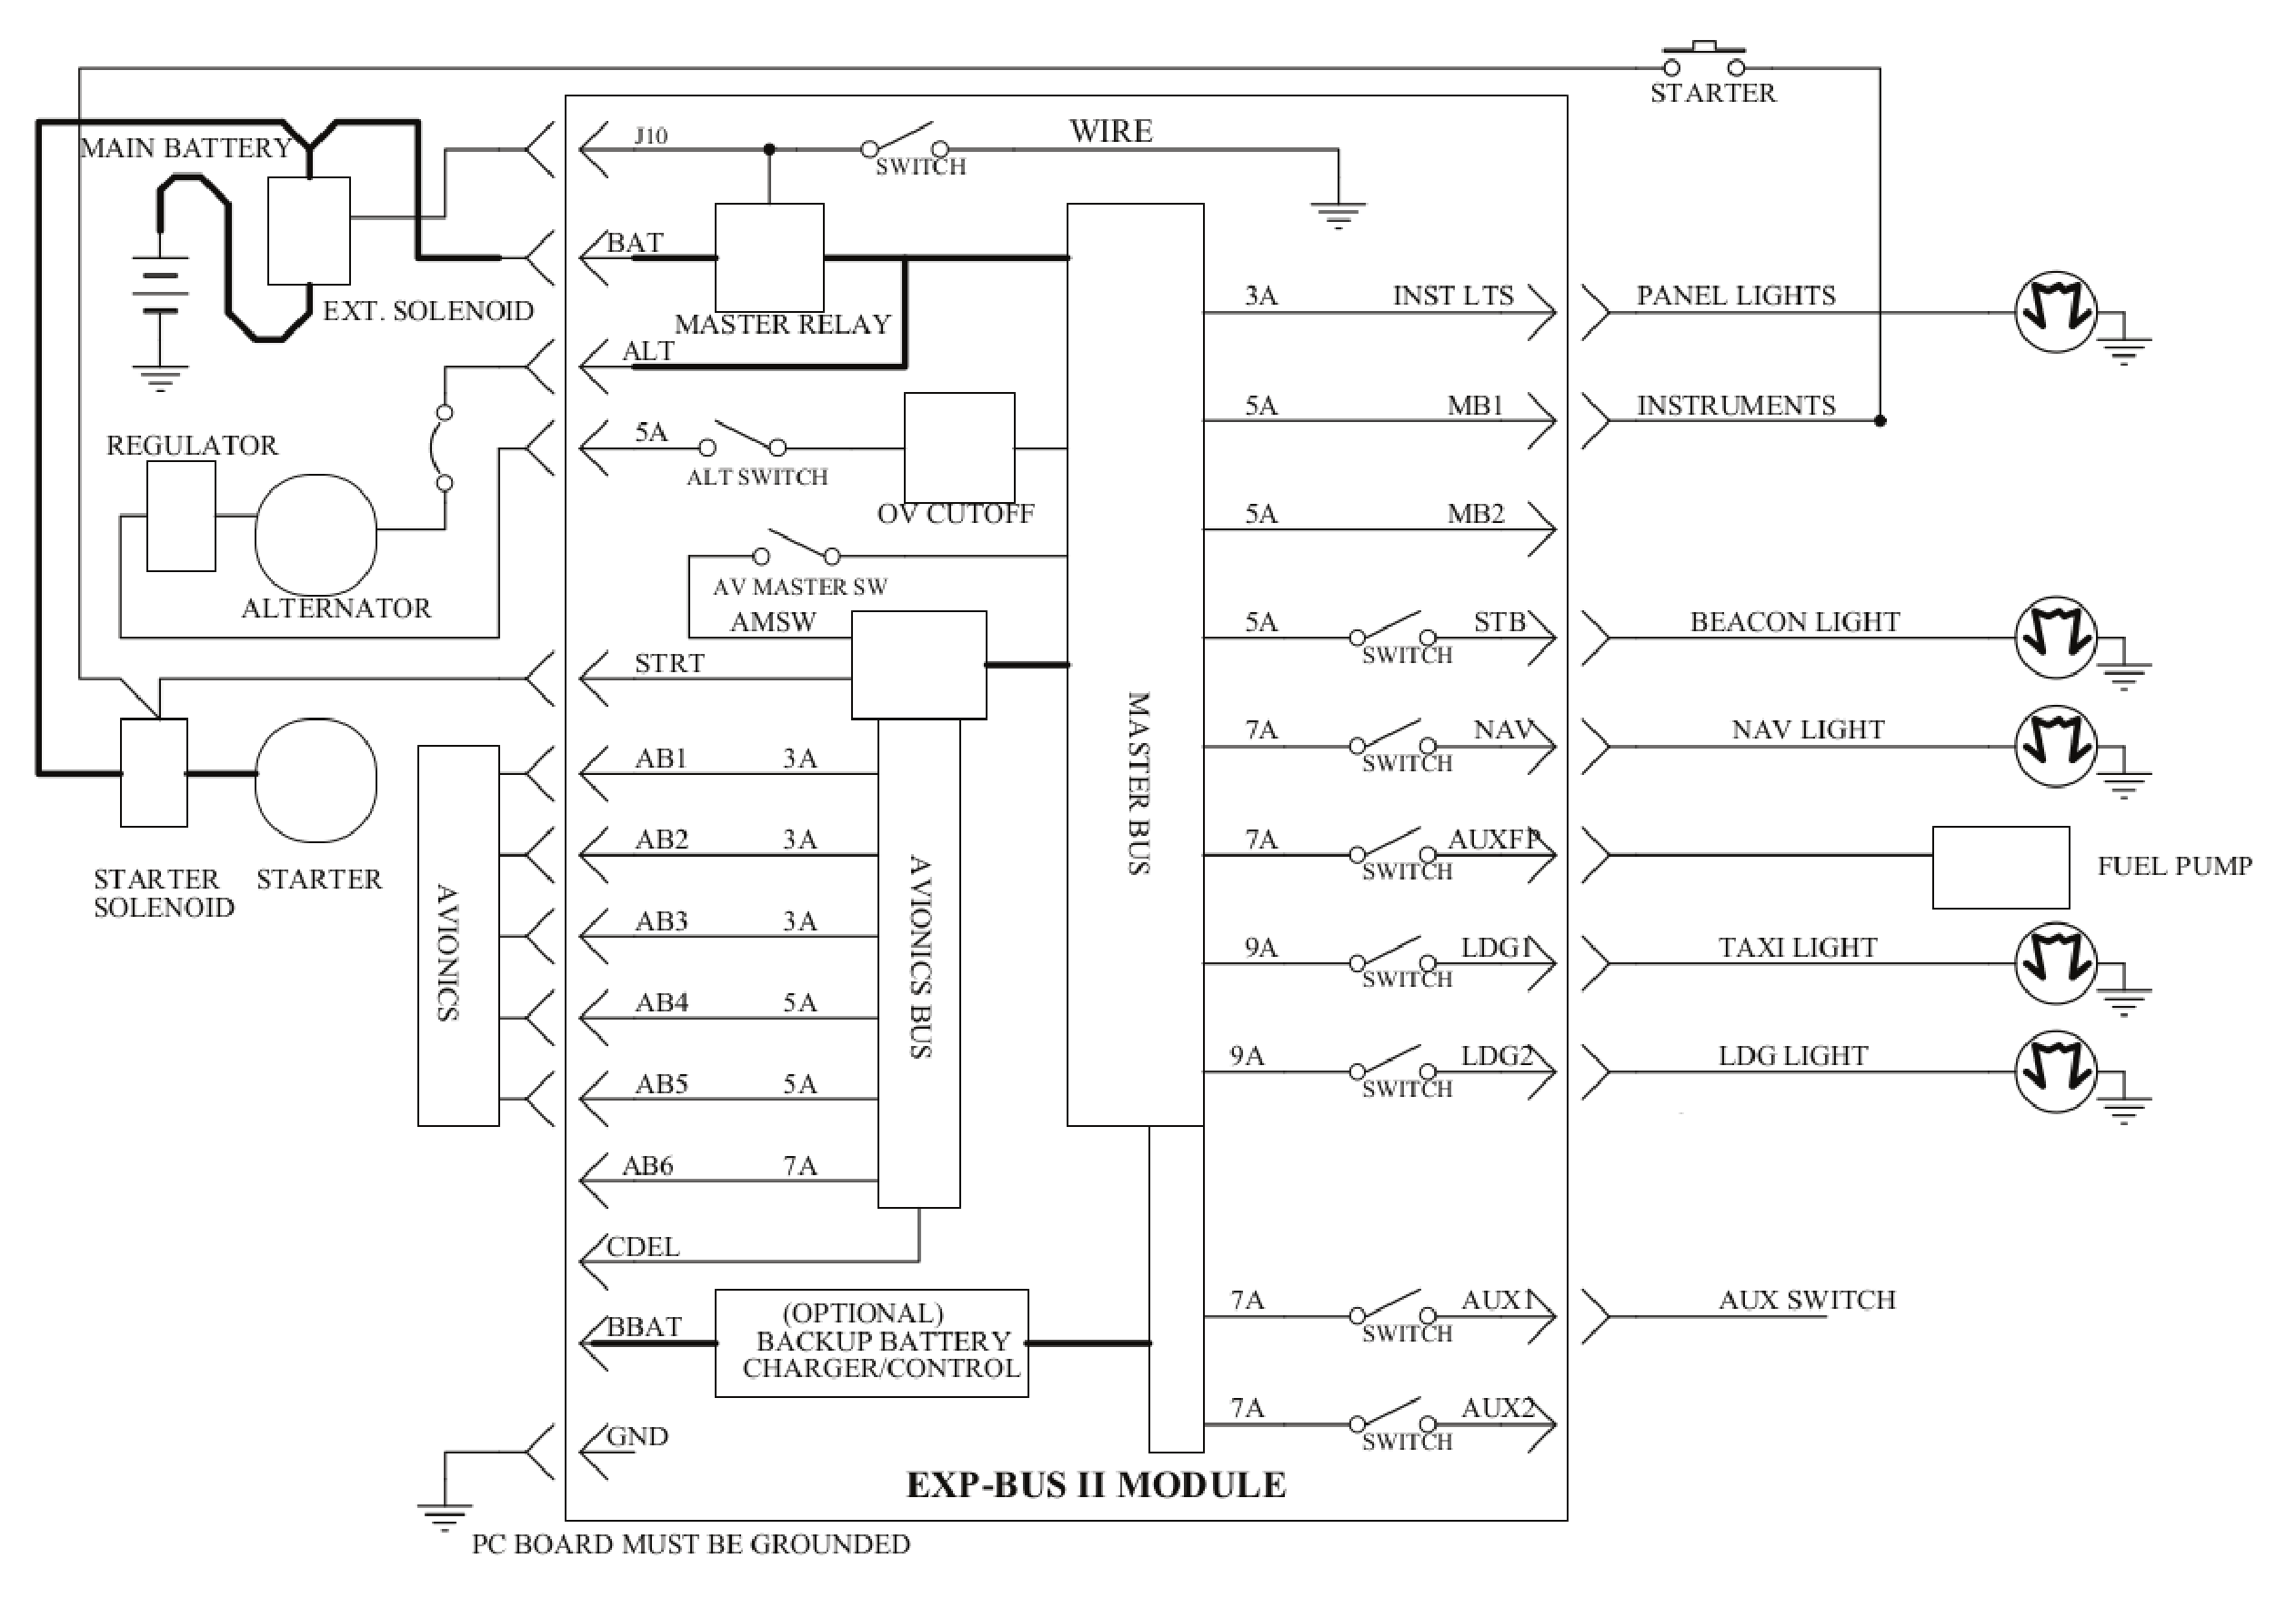
\includegraphics[height=0.6\textheight]{elec_block.eps}
\caption{Electrical system block diagram}
\label{fig:electrical}
\end{figure}
\end{sidewaysfigure}

The electrical system includes a 14 volt 60 amp alternator with an internal regulator and overvoltage protection.

The alternator is protected from overload by a 60A fuse mounted on the engine firewall. The main aircraft battery
is a 12-volt sealed Odyssey battery, which is mounted on the right side of the forward firewall just above the
main battery and starter relays.

The aircraft has no conventional circuit breakers but is instead fitted with an EXP BUS DC load centre which
makes use of solid state current limiting devices known as PTC current limiters. These devices have unique
advantages over fuses and circuit breakers. 

Like a fuse, the PTC device 'blows' when too much current is drawn by an offending circuit, however, like a circuit breaker, the PTC can be reset and in fact does this automatically once the load is COMPLETELY removed.

To reset a circuit simply switch the item off and wait about ten to fifteen seconds for the PTC to reset. Should the
fault have cleared, the circuit will be restored when the switch is turned back on.

The alternator field switch is located next to the master switch. This switch will be disabled should the bus voltage exceed 18V.

Electrical accessories include starter, electric fuel pump, flap actuator, exterior lights, trim motors and avionics
as listed in the equipment section.

\section{Instruments}
The aircraft is fitted with a MGL Odyssey EFIS system as its Primary Flight Display and Engine
Management System. The EFIS unit is powered from a dedicated power switch on the instrument panel.  

A system backup battery is mounted behind the EFIS display and is able to hold configuration data only.  

The MGL RDAC engine module is mounted forward of the firewall under the engine cowl and provides the interface between the EFIS and the engine. 

The MGL ADAHRS is mounted in front of the fuel selector switch on top of the fuel pump cover.  
The MGL magnetometer is mounted behind the baggage area bulkhead.  

Outside Air Temperature is obtained from a sensor mounted on the left bottom cockpit behind the pilot rudder pedals.

A standby analogue airspeed indicator and altimeter are fitted for redundancy.

\section{Avionics}
The following aircraft avionics is fitted and powered once the avionics switch is on:
\begin{itemize}
\item The GARMIN GX 327 is a mode C transponder.
\item MGL V6 COM radio
\item Microair COM radio
\end{itemize}

A GPS antenna is mounted on top of the engine mount underneath the top engine cowl.  

\section{Heating and Ventilation}
Cabin heat is provided via a heat muff attached to the exhaust system and fed with high-pressure air from the front
right engine baffle plate. Flow of hot air enters through a valve on the lower centre and is controlled with a
ratchet cable and knob marked CABIN HEAT. Flow is off in the forward position. When in the OFF position, air
passing through the muff and ducts is dumped into the low-pressure section of the cowl.

Fresh air from naca ducts on the forward side of the fuselage is fed into vents on either side of the instrument
panel for front occupants.


\subsection{Canopy and cabin features}
The canopy is unlatched using the handle on the top middle of the canopy.  To open the canopy should be rolled back while lifting the back slightly to ease it up on the guide rail.  

Entry into the cabin is made by first stepping on the wing, taking care not to step onto the flaps.  The area on the wing where it is safe to stand is covered in black non-slip \textit{wingwalk} material.  From the wing step onto the seat over the cabin side and then slide down into a seated position.

The pilot and passenger backrest may be adjusted forward and aft by means of a piano hinge style system.  The backrest may also be angled to more than one position. 

Both seats are fitted with a four-point harness, which should be carefully fitted and adjusted prior to take off. In single person operations the unused straps should be used to secure the seat cushions and to prevent the straps flying about.
Straps should be checked regularly for damage.

\subsection{Baggage space and entry dimensions}
The baggage area is located behind the passenger seat backrests.  The baggage area has a maximum load capacity of 100 lbs and volume of 12 cubic feet.  

 Baggage needs to be lifted over the seatbacks and fit under the rolled back canopy.  This will constrain the maximum dimension of any item in the baggage area.


\chapter{Service and Maintenance}
\thispagestyle{fancy}
\minitoc[n] % Creating an actual minitoc

\section{General}
This section provides information on handling, service and maintenance of the aircraft.

The owner can obtain up-to-date service bulletins from the Van’s web site at www.vansaircraft.com. 
Service bulletins on the Lycoming Kit engine can be obtained from www.lycoming.com and any information relating to the installed propeller from the Hartzell
manufacturer at www.hartzellprop.com.

The South African CAA or the Aero Club of South Africa may also issue information and directives. These
directives could be advisory or mandatory. As failure to implement such a directive could contravene the
issued Permit to Fly (as well as risking safety) It is essential the owner keep up to date on all such
relevant information relating to the aircraft, and its installed systems equipment.

\section{Ground Handling}
Ground towing/non-taxi movement can be accomplished by manoeuvring with the castoring tail wheel.  When
taxiing the aircraft ensure that the taxi path and propeller back blast areas are clear. In the first few feet of taxi
apply the brakes to ensure effectiveness. Do not operate the engine at high rpm, taxi with care
When parking, ensure aircraft is  protected from adverse weather and that it presents no danger to
others. Park the aircraft into wind if possible and tie down securely.


\section{Maintenance and Service}
Refer to the Reference section for 50/100hr/annual maintenance requirements and overhaul time periods.

All work should be entered in the appropriate log book indicating:-
\begin{itemize}
  \item Date work was done
  \item Description of work 
  \item Number of hours recorded on the aircraft at that time.
  \item Name and signature of individual doing the work.
\end{itemize}

\subsection{25 Hour Inspection}
The following 25-hour check is in essence a detailed pre-flight developed from relevant sources and based on best practice. 

\subsubsection{Engine compartment}
Remove engine cowls for general inspection including the following: 
\begin{enumerate}
\item Oil hoses and filter. Check for leaks and security.
\item Oil cooler. General check of installation
\item Oil. Check level and review top up frequency
\item Induction filter. Check filter visually
\item Fuel injection servo/Carburettor. General exterior check including control cables.
\item Magneto. General exterior inspection and security
\item Plug leads. Inspect for condition
\item Fuel hoses. Check for leaks and signs of loosening
\item Fuel pump. Check body joins for leaks
\item Exhaust system. Check for blowing manifold gaskets
\item Check heat muffs and ducting
\item Check joints for wear/damage. Check mounting points
\item Check general integrity of system
\item Engine mount. Check for damage
\item Brake fluid. Check level, note change since last service.
\item Compartment wiring. Check for damage and security.
\item Cooling system. Check for damage/wear/security.
\item Check baffles and flexible sealing strips.
\item General. Review/inspection of engine compartment
\item Cowls. Inspect for damage.
\item Replace cowls
\end{enumerate}
\subsubsection{Propeller inspection}
\begin{enumerate}
\item Propeller. Check for nicks, scratches, leaks or corrosion.
\item Spinner. Check spinner and back plate for condition.
\end{enumerate}
\subsubsection{External inspection}
\begin{enumerate}
\item Remove all wheel spats:
\item Tyres. Check pressures, mains  30-35 psi. (Cold) %and nose
\item Inspect tyres for wear and slip on hub.
\item Brake system. Inspect brake pads, replace if appropriate.
\item Inspect hydraulic lines, joints and bleed points.
\item Wheels. Check bearings for play. Check split pins and bolts for security, including the split-hub bolts.
\item Spats. Inspect for damage, replace wheel spats.
\item General airframe and control surfaces review including, but not limited to:
\item Control surfaces. Individual inspection of each surface for free movement, satisfactory mounting/hinge condition
and actuating system integrity, particular attention should be given to flap actuating rods as the rod end is not
safe tied.
\item Fibreglass components. General inspection for integrity.
\item Fuel tanks. Inspect for leaks and security.
\end{enumerate}


\section{Propeller Maintenance}
\subsection{Lubrication Intervals}
\begin{enumerate}
\item 
The propeller must be lubricated at intervals not to 
exceed 100 hours or at 12 calendar months, whichever 
occurs first.
\subitem
If annual operation is significantly less than 100 
hours, calendar lubrication intervals should be 
reduced to six months.
\subitem
If the aircraft is operated or stored under adverse 
atmospheric conditions, e.g., high humidity, salt air, 
calendar lubrication intervals should be reduced to 
six months.
\item
Owners of high use aircraft may wish to extend their 
lubrication interval. Lubrication interval may be gradually 
extended after evaluation of previous propeller overhauls 
with regard to bearing wear and internal corrosion.
\item 
Hartzell Propeller Inc. recommends that new or newly 
overhauled propellers be lubricated after the first one or 
two hours of operation because centrifugal loads will pack 
and redistribute grease, which may result in a propeller 
imbalance. Redistribution of grease may also result in 
voids in the blade bearing area where moisture can collect.
\end{enumerate}

\section{Battery Maintenance}
The State of Charge of the battery can be determined from Figure~\ref{fig:SOC}.

\begin{figure}[H]
\centering
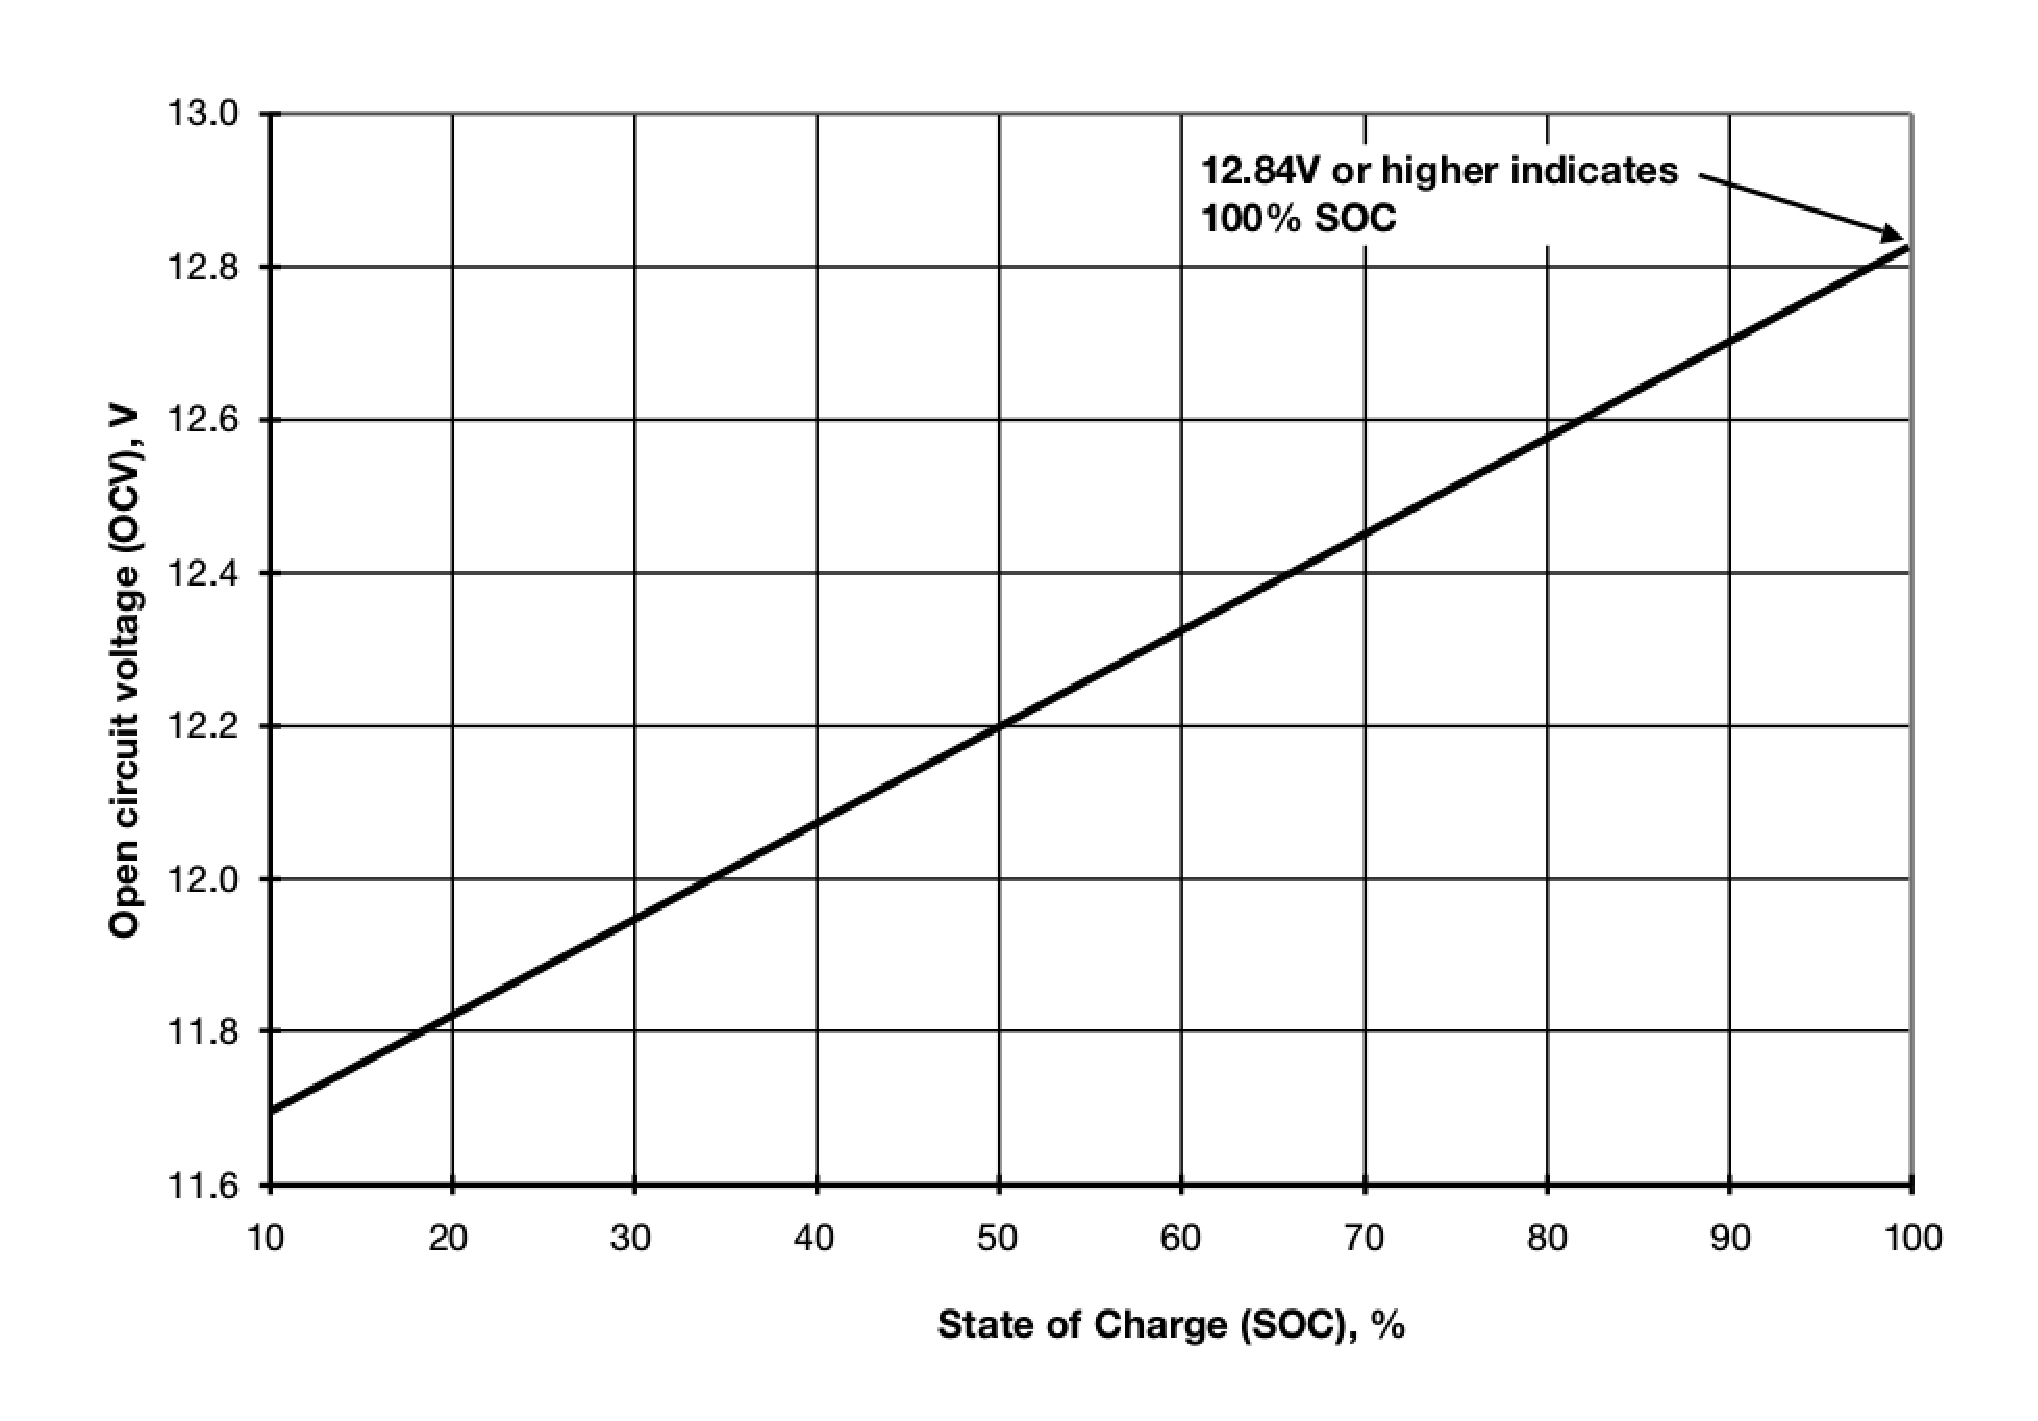
\includegraphics[height=0.7\textwidth]{stateofcharge.eps}
\caption{State of Charge}
\label{fig:SOC}
\end{figure}

To get long life from the battery, it is important that the battery is kept near full charge, approximately 12.8V.  If there are electrical loads douring storage, then the negative battery cable should be disconnected OR an independent float charger used.

%\chapter{Supplements}
\thispagestyle{fancy}
\minitoc[n] % Creating an actual minitoc

\section{Introduction}
Section 2 includes operating limitations, instrument markings and basic placards necessary for the safe operation of the airplne, its engine, standard systems and standard equipment.

\section{Airspeed Limitations}


\begin{center}
\begin{tabular}{ |p{1cm}|p{6cm}|p{2cm}|p{5cm}| } 
 \hline
  & SPEEDS &  KIAS & REMARKS\\ 
 \hline
 $V_{NE}$ & Never exceed speed & 200 & Do not exceed this speed in any operation\\ 
 \hline
 $V_{NO}$ & Maximum structural cruising speed & 168  & Do not exceed this speed except in smooth air, and then only with caution\\ 
 \hline
 $V_{A}$ & Maneuvering Speed & 123  & Do not make full or abrupt control movements above this speeds \\ 
 \hline
 $V_{FE}$  & \shortstack[l]{Maximum Flap Extended Speed: \\To 20$^{\circ}$ Flaps\\ 20$^{\circ}$ - 40$^{\circ}$ Flaps} & \shortstack[l]{\\96 \\ 87} & Do not exceed these speeds with the given flap settings \\ 
 \hline
\end{tabular}
\end{center}



\end{document}
\grid
